% Seminarul 5: Volatilitate condiționată: ARCH și GARCH
% Serii de timp -- Programele de licență Informatică economică și Cibernetică economică, Academia de Studii Economice din București
% GENERAT de latex/build_seminar5.py -- modificați generatorul, nu acest fișier.
% Implicit versiunea pentru studenți; versiunea profesorului este wrapper-ul *_solutions.tex.
\makeatletter\@ifundefined{ifsolutions}{\expandafter\newif\csname ifsolutions\endcsname}{}\makeatother

\newcommand{\coursename}{Serii de timp}
\def\tsalang{ro}
% Preambul comun TSA -- Serii de timp / Time Series Analysis (Beamer, 16:9)
% Același design ca MFM și SFM (preluat din SFM, 5 octombrie 2026). Înainte de % Preambul comun TSA -- Serii de timp / Time Series Analysis (Beamer, 16:9)
% Același design ca MFM și SFM (preluat din SFM, 5 octombrie 2026). Înainte de % Preambul comun TSA -- Serii de timp / Time Series Analysis (Beamer, 16:9)
% Același design ca MFM și SFM (preluat din SFM, 5 octombrie 2026). Înainte de \input{../../latex/preamble} se definește
%   \newcommand{\coursename}{Time Series Analysis}      (EN)
%   \newcommand{\coursename}{Serii de timp}       (RO)  și  \def\tsalang{ro}
% Fișierele .tex se află în EN/Courses, EN/Seminars, RO/Cursuri, RO/Seminarii (două niveluri sub rădăcină).
% Deck-urile sînt generate de latex/build_chapterN.py / build_seminarN.py (vezi latex/tsa_build.py).

\documentclass[9pt, aspectratio=169, t]{beamer}
\providecommand{\coursename}{Time Series Analysis}

% Ensure content fits on slides
\setbeamersize{text margin left=8mm, text margin right=8mm}
% Smaller institute font (title page)
\setbeamerfont{institute}{size=\footnotesize}

%=============================================================================
% THEME AND STYLE CONFIGURATION
%=============================================================================
\usetheme{default}
% Using default theme for clean header/footer control

% Color Palette (matching Redispatch PDF)
\definecolor{MainBlue}{RGB}{26, 58, 110}
\definecolor{AccentBlue}{RGB}{26, 58, 110}
\definecolor{IDAred}{RGB}{205, 0, 0}
\definecolor{DarkGray}{RGB}{51, 51, 51}
\definecolor{MediumGray}{RGB}{128, 128, 128}
\definecolor{LightGray}{RGB}{248, 248, 248}
\definecolor{VeryLightGray}{RGB}{235, 235, 235}
\definecolor{KeynoteGray}{RGB}{218, 218, 218}
\definecolor{SectionGray}{RGB}{120, 120, 120}
\definecolor{FooterGray}{RGB}{100, 100, 100}
\definecolor{Crimson}{RGB}{220, 53, 69}
\definecolor{Forest}{RGB}{46, 125, 50}
\definecolor{Amber}{RGB}{181, 133, 63}
\definecolor{Orange}{RGB}{230, 126, 34}
\definecolor{Purple}{RGB}{142, 68, 173}

% Gradient background (exact Keynote 315° gradient: white to RGB 218,218,218)
\setbeamertemplate{background}{%
    \begin{tikzpicture}[remember picture, overlay]
        \shade[shading=axis, shading angle=315,
        top color=white, bottom color=KeynoteGray]
        (current page.south west) rectangle (current page.north east);
    \end{tikzpicture}%
}
% Fallback solid color for compatibility
\setbeamercolor{background canvas}{bg=}

\setbeamercolor{palette primary}{bg=MainBlue, fg=white}
\setbeamercolor{palette secondary}{bg=MainBlue!85, fg=white}
\setbeamercolor{palette tertiary}{bg=MainBlue!70, fg=white}
\setbeamercolor{structure}{fg=MainBlue}
\setbeamercolor{title}{fg=IDAred}
\setbeamercolor{frametitle}{fg=IDAred, bg=}
\setbeamercolor{block title}{bg=MainBlue, fg=white}
\setbeamercolor{block body}{bg=VeryLightGray, fg=DarkGray}
\setbeamercolor{block title alerted}{bg=Crimson, fg=white}
\setbeamercolor{block body alerted}{bg=Crimson!8, fg=DarkGray}
\setbeamercolor{block title example}{bg=Forest, fg=white}
\setbeamercolor{block body example}{bg=Forest!8, fg=DarkGray}
\setbeamercolor{item}{fg=MainBlue}

% Footer colors (override Madrid theme blue)
\setbeamercolor{author in head/foot}{fg=FooterGray, bg=}
\setbeamercolor{title in head/foot}{fg=FooterGray, bg=}
\setbeamercolor{date in head/foot}{fg=FooterGray, bg=}
\setbeamercolor{section in head/foot}{fg=FooterGray, bg=}
\setbeamercolor{subsection in head/foot}{fg=FooterGray, bg=}

% Bullet styles (apply everywhere including blocks)
\setbeamertemplate{itemize item}{\color{MainBlue}$\boxdot$}
\setbeamertemplate{itemize subitem}{\color{MainBlue}$\blacktriangleright$}
\setbeamertemplate{itemize subsubitem}{\color{MainBlue}\tiny$\bullet$}
\setbeamertemplate{itemize/enumerate body begin}{\normalsize}
\setbeamertemplate{itemize/enumerate subbody begin}{\normalsize}

% Item spacing - compact style
\setlength{\leftmargini}{10pt}       % Level 1: minimal indent
\setlength{\leftmarginii}{10pt}      % Level 2: minimal additional indent
% Compact list spacing (zero extra space before/after lists in blocks)
\makeatletter
\def\@listi{\leftmargin\leftmargini \topsep 0pt \parsep 0pt \itemsep 0pt}
\def\@listii{\leftmargin\leftmarginii \topsep 0pt \parsep 0pt \itemsep 0pt}
\makeatother

\setbeamertemplate{navigation symbols}{}

%=============================================================================
% CUSTOM HEADLINE
%=============================================================================
\setbeamertemplate{headline}{%
    \vskip10pt%
    \hbox to \paperwidth{%
        \hskip0.5cm%
        {\small\color{FooterGray}\renewcommand{\hyperlink}[2]{##2}\insertsectionhead}%
        \hfill%
        \textcolor{FooterGray}{\small\insertframenumber}%
        \hskip0.5cm%
    }%
    \vskip4pt%
    {\color{FooterGray}\hrule height 0.4pt}%
}

%=============================================================================
% CUSTOM FOOTER
%=============================================================================
\usepackage{fontawesome5}

\setbeamertemplate{footline}{%
    {\color{FooterGray}\hrule height 0.4pt}%
    \vskip4pt%
    \hbox to \paperwidth{%
        \hskip0.5cm%
        \textcolor{FooterGray}{\small\coursename}%
        \hfill%
        \raisebox{-0.1em}{%
            \begin{tikzpicture}[x=0.08em, y=0.08em, line width=0.4pt]
                \draw[FooterGray] (0,3) -- (1,4) -- (2,3.5) -- (3,5) -- (4,4) -- (5,6) -- (6,5.5) -- (7,4) -- (8,5) -- (9,7) -- (10,6) -- (11,5) -- (12,6.5) -- (13,8) -- (14,7) -- (15,6) -- (16,7.5) -- (17,9) -- (18,8) -- (19,7) -- (20,8.5) -- (21,10) -- (22,9) -- (23,8) -- (24,9.5);
            \end{tikzpicture}%
        }%
        \hskip0.5cm%
    }%
    \vskip6pt%
}

%=============================================================================
% PACKAGES
%=============================================================================
\usepackage[utf8]{inputenc}
\DeclareUnicodeCharacter{03B1}{\ensuremath{\alpha}}
\usepackage[T1]{fontenc}
\usepackage{amsmath, amssymb, amsthm}
\usepackage{mathtools}
\usepackage{bm}
\usepackage{tikz}
\usetikzlibrary{arrows.meta, positioning, shapes, calc, decorations.pathreplacing, shadings}
\usepackage{booktabs}
\usepackage{multirow}
\usepackage{array}
\usepackage{graphicx}
\usepackage{animate}
\usepackage{hyperref}
\usepackage{colortbl}
\usepackage{listings}
\lstset{language=Python, basicstyle=\ttfamily\scriptsize, keywordstyle=\color{MainBlue}\bfseries,
  commentstyle=\color{Forest}, stringstyle=\color{Crimson}, breaklines=true,
  frame=none, backgroundcolor=\color{VeryLightGray}, xleftmargin=2mm}
\hypersetup{colorlinks=true, linkcolor=MainBlue, urlcolor=MainBlue}
\graphicspath{{../../logos/}{../../charts/}{../../photos/}}
\usepackage{xcolor}
\hfuzz=2pt  % Suppress tiny overfull warnings (<2pt)
\vfuzz=2pt  % Suppress tiny vertical overfull warnings (<2pt)
% \mathrm in the sans-serif family of the slides (beamer resets \mathrm to the serif family at \begin{document};
% this hook runs after beamer's, so WN, Var, RMSE, ... in formulas match the surrounding text)
% Bold vectors and matrices in the same sans-serif family: \mathbf{A} in sans bold (beamer's own \mathbf came out in
% medium weight), and the bold upright Greek capitals of \boldsymbol / \bm (\bSigma, \bPhi, \boldsymbol{\Theta}) in
% cmss bold: bm.sty fixes its "boldoperators" font when it is loaded (serif cmbx), before beamer switches the
% operators to cmss, so it is reset here.
\AtBeginDocument{%
  \SetMathAlphabet{\mathrm}{normal}{\encodingdefault}{\sfdefault}{\mddefault}{n}%
  \SetMathAlphabet{\mathrm}{bold}{\encodingdefault}{\sfdefault}{bx}{n}%
  \SetMathAlphabet{\mathbf}{normal}{\encodingdefault}{\sfdefault}{bx}{n}%
  \SetMathAlphabet{\mathbf}{bold}{\encodingdefault}{\sfdefault}{bx}{n}%
  \SetSymbolFont{boldoperators}{normal}{OT1}{cmss}{bx}{n}%
  \SetSymbolFont{boldoperators}{bold}{OT1}{cmss}{bx}{n}}

%=============================================================================
% QUANTLET COMMANDS
%   \quantlet{<displayed name>}{<url>}       (generic, compatible with the older TSA decks)
%   \tsaquantlet{Ch_05}{TSA_ch5_garch}       -> https://github.com/danpele/Time-Series-Analysis/tree/main/Quantlets/Ch_05/TSA_ch5_garch
%   \qlurl{<folder>} is defined per chapter by the generator (Quantlets/Ch_NN/<folder>)
%=============================================================================
\newcommand{\tsarepo}{https://github.com/danpele/Time-Series-Analysis}
\newcommand{\tsaqlbase}{https://github.com/danpele/Time-Series-Analysis/tree/main/Quantlets}
\newcommand{\quantlet}[2]{%
    \hfill\href{#2}{%
        \raisebox{-0.15em}{
\includegraphics[height=0.7em]{ql_logo.png}}%
        \textcolor{MainBlue}{\tiny\ #1}%
    }%
}
\newcommand{\tsaquantlet}[2]{\quantlet{\detokenize{#2}}{\tsaqlbase/#1/#2}}

%=============================================================================
% NOTEBOOKS (Google Colab)
%   \colaburl{notebooks/EN/chapter5_seminar_notebook.ipynb} -> the Colab link of a file in the TSA repo
%   \nb: the chapter notebook (each seminar deck redefines it with \renewcommand)
%=============================================================================
\newcommand{\colaburl}[1]{https://colab.research.google.com/github/danpele/Time-Series-Analysis/blob/main/#1}
\newcommand{\nb}{https://colab.research.google.com/github/danpele/Time-Series-Analysis/tree/main/notebooks/EN}
\newcommand{\nbname}{notebooks/EN}

%=============================================================================
% SLIDE HELPERS (used by the generators; the same as in MFM)
%=============================================================================
% local font size for list bodies (the preamble forces \normalsize)
\newcommand{\itemsize}[1]{\setbeamertemplate{itemize/enumerate body begin}{#1}\setbeamertemplate{itemize/enumerate subbody begin}{#1}}
\newcommand{\intitle}[1]{{\hypersetup{urlcolor=white}#1}}   % white links inside coloured title bars
\newcommand{\imgcap}[1]{{\scriptsize #1}\\[0.5mm]}          % caption under a photo
\newcommand{\imgcredit}[2]{{\tiny\color{FooterGray}\href{#1}{#2}}}   % image credit: source URL, author/licence
\newcommand{\aiprompt}[1]{{\ttfamily\color{MainBlue}#1}}     % a prompt to an AI assistant

%=============================================================================
% SEMINARS: student version by default; the instructor wrapper *_solutions.tex sets \solutionstrue
%=============================================================================
\makeatletter\@ifundefined{ifsolutions}{\expandafter\newif\csname ifsolutions\endcsname}{}\makeatother
\newcommand{\solonly}[1]{\ifsolutions #1\fi}
\newcommand{\propsub}{\ifsolutions\else\framesubtitle{\ifdefined\tsalang Rezolvarea se discută la seminar\else Solution discussed in class\fi}\fi}

%=============================================================================
% APPENDIX AND CHAPTER LINKS (latex/appendix_links.py writes the calls; it also re-declares these
% macros before \begin{document}, so the decks compile with or without this preamble block)
%=============================================================================
\providecommand{\tsaapplink}[3]{\hypertarget{#2}{}\hyperlink{#1}{\beamergotobutton{#3}}}
\providecommand{\tsaappback}[2]{\begin{tikzpicture}[remember picture,overlay]\node[anchor=south east] at ([xshift=-3mm,yshift=7mm]current page.south east){\hyperlink{#1}{\beamerreturnbutton{#2}}};\end{tikzpicture}}
\providecommand{\tsachlink}[2]{\href{#1}{#2}}
\providecommand{\tsachlinkt}[2]{\href{#1}{\usebeamercolor[fg]{frametitle}#2}}

%=============================================================================
% QUANTINAR COMMAND: link către un curs Quantinar (subiecte avansate)
%=============================================================================
\newcommand{\quantinar}[2]{%
    \href{#2}{%
        \raisebox{-0.15em}{
\includegraphics[height=0.8em]{qr_logo.png}}%
        \textcolor{MainBlue}{\scriptsize\ #1}%
    }%
}

%=============================================================================
% CUSTOM TITLE PAGE
%=============================================================================
\defbeamertemplate*{title page}{hybrid}[1][]
{
    \vspace{0.2cm}
    % Logos row - top header (with clickable links)
    \begin{center}
        \href{https://www.ase.ro}{
\includegraphics[height=1.0cm]{ase_logo.png}}\hspace{0.3cm}%
        \href{https://theida.net}{
\includegraphics[height=1.0cm]{ida_logo.png}}\hspace{0.3cm}%
        \href{https://blockchain-research-center.com}{
\includegraphics[height=1.0cm]{brc_logo.png}}\hspace{0.3cm}%
        \href{https://www.ai4efin.ase.ro}{
\includegraphics[height=1.0cm]{ai4efin_logo.png}}\hspace{0.3cm}%
        \href{https://ipe.ro/new}{
\includegraphics[height=1.0cm]{acad_logo.png}}\hspace{0.3cm}%
        \href{https://www.digital-finance-msca.com}{
\includegraphics[height=1.0cm]{msca_logo.png}}%
    \end{center}

    \vspace{0.6cm}

    % Main title with Q logos on sides (with clickable links)
    \begin{center}
        \begin{minipage}{0.1\textwidth}
            \centering
            \href{https://quantlet.com}{
\includegraphics[height=1.1cm]{ql_logo.png}}
        \end{minipage}%
        \begin{minipage}{0.78\textwidth}
            \centering
            {\LARGE\bfseries\usebeamercolor[fg]{title}\inserttitle}

            \vspace{0.3cm}

            {\usebeamerfont{subtitle}\usebeamercolor[fg]{title}\insertsubtitle}
        \end{minipage}%
        \begin{minipage}{0.1\textwidth}
            \centering
            \href{https://quantinar.com}{
\includegraphics[height=1.1cm]{qr_logo.png}}
        \end{minipage}
    \end{center}

    \vspace{0.6cm}

    % Authors (left aligned)
    \hspace{0.5cm}{\usebeamerfont{author}\insertauthor}

    \vspace{0.3cm}

    % Institute/Affiliations (left aligned)
    \hspace{0.5cm}\begin{minipage}[t]{0.9\textwidth}
        \raggedright\small\insertinstitute
    \end{minipage}
}

%=============================================================================
% THEOREM ENVIRONMENTS
%=============================================================================
\theoremstyle{definition}
\setbeamertemplate{theorems}[numbered]
\ifdefined\tsalang
\newtheorem{defn}{Definiție}
\newtheorem{thm}{Teoremă}
\newtheorem{prop}{Propoziție}
\newtheorem{rmk}{Observație}
\else
\newtheorem{defn}{Definition}
\newtheorem{thm}{Theorem}
\newtheorem{prop}{Proposition}
\newtheorem{rmk}{Remark}
\fi

%=============================================================================
% CENTRED MINIPAGE (no extra vertical space)
%=============================================================================
\newenvironment{cminipage}[1]{%
    \par\noindent\hfill\begin{minipage}{#1}\ignorespaces
}{%
    \end{minipage}\hfill\null\par
}

%=============================================================================
% CUSTOM COMMANDS
%=============================================================================
\newcommand{\E}{\mathbb{E}}
\newcommand{\Var}{\text{Var}}
\newcommand{\Cov}{\text{Cov}}
\newcommand{\Corr}{\text{Corr}}
\newcommand{\R}{\mathbb{R}}
\newcommand{\N}{\mathbb{N}}
\newcommand{\Z}{\mathbb{Z}}
\newcommand{\B}{\mathbf{B}}
\newcommand{\imark}{\textcolor{MainBlue}{\textbullet}}
\newcommand{\RMSE}{\text{RMSE}}
\newcommand{\MAE}{\text{MAE}}
\newcommand{\MAPE}{\text{MAPE}}

% Boldface vector/matrix commands (VAR, VECM, state space; also used by the older TSA decks)
\newcommand{\bY}{\mathbf{Y}}
\newcommand{\bX}{\mathbf{X}}
\newcommand{\bA}{\mathbf{A}}
\newcommand{\bB}{\mathbf{B}}
\newcommand{\bepsilon}{\boldsymbol{\varepsilon}}
\newcommand{\bSigma}{\boldsymbol{\Sigma}}
\newcommand{\bPhi}{\boldsymbol{\Phi}}
\newcommand{\bGamma}{\boldsymbol{\Gamma}}
\newcommand{\bPi}{\boldsymbol{\Pi}}
\newcommand{\bc}{\mathbf{c}}
\newcommand{\balpha}{\boldsymbol{\alpha}}
\newcommand{\bbeta}{\boldsymbol{\beta}}
\newcommand{\bvarepsilon}{\boldsymbol{\varepsilon}}

% Legacy seminar marks (older TSA seminar decks)
\newcommand{\correct}{\textcolor{Forest}{\checkmark}}
\newcommand{\incorrect}{\textcolor{Crimson}{\texttimes}}
 se definește
%   \newcommand{\coursename}{Time Series Analysis}      (EN)
%   \newcommand{\coursename}{Serii de timp}       (RO)  și  \def\tsalang{ro}
% Fișierele .tex se află în EN/Courses, EN/Seminars, RO/Cursuri, RO/Seminarii (două niveluri sub rădăcină).
% Deck-urile sînt generate de latex/build_chapterN.py / build_seminarN.py (vezi latex/tsa_build.py).

\documentclass[9pt, aspectratio=169, t]{beamer}
\providecommand{\coursename}{Time Series Analysis}

% Ensure content fits on slides
\setbeamersize{text margin left=8mm, text margin right=8mm}
% Smaller institute font (title page)
\setbeamerfont{institute}{size=\footnotesize}

%=============================================================================
% THEME AND STYLE CONFIGURATION
%=============================================================================
\usetheme{default}
% Using default theme for clean header/footer control

% Color Palette (matching Redispatch PDF)
\definecolor{MainBlue}{RGB}{26, 58, 110}
\definecolor{AccentBlue}{RGB}{26, 58, 110}
\definecolor{IDAred}{RGB}{205, 0, 0}
\definecolor{DarkGray}{RGB}{51, 51, 51}
\definecolor{MediumGray}{RGB}{128, 128, 128}
\definecolor{LightGray}{RGB}{248, 248, 248}
\definecolor{VeryLightGray}{RGB}{235, 235, 235}
\definecolor{KeynoteGray}{RGB}{218, 218, 218}
\definecolor{SectionGray}{RGB}{120, 120, 120}
\definecolor{FooterGray}{RGB}{100, 100, 100}
\definecolor{Crimson}{RGB}{220, 53, 69}
\definecolor{Forest}{RGB}{46, 125, 50}
\definecolor{Amber}{RGB}{181, 133, 63}
\definecolor{Orange}{RGB}{230, 126, 34}
\definecolor{Purple}{RGB}{142, 68, 173}

% Gradient background (exact Keynote 315° gradient: white to RGB 218,218,218)
\setbeamertemplate{background}{%
    \begin{tikzpicture}[remember picture, overlay]
        \shade[shading=axis, shading angle=315,
        top color=white, bottom color=KeynoteGray]
        (current page.south west) rectangle (current page.north east);
    \end{tikzpicture}%
}
% Fallback solid color for compatibility
\setbeamercolor{background canvas}{bg=}

\setbeamercolor{palette primary}{bg=MainBlue, fg=white}
\setbeamercolor{palette secondary}{bg=MainBlue!85, fg=white}
\setbeamercolor{palette tertiary}{bg=MainBlue!70, fg=white}
\setbeamercolor{structure}{fg=MainBlue}
\setbeamercolor{title}{fg=IDAred}
\setbeamercolor{frametitle}{fg=IDAred, bg=}
\setbeamercolor{block title}{bg=MainBlue, fg=white}
\setbeamercolor{block body}{bg=VeryLightGray, fg=DarkGray}
\setbeamercolor{block title alerted}{bg=Crimson, fg=white}
\setbeamercolor{block body alerted}{bg=Crimson!8, fg=DarkGray}
\setbeamercolor{block title example}{bg=Forest, fg=white}
\setbeamercolor{block body example}{bg=Forest!8, fg=DarkGray}
\setbeamercolor{item}{fg=MainBlue}

% Footer colors (override Madrid theme blue)
\setbeamercolor{author in head/foot}{fg=FooterGray, bg=}
\setbeamercolor{title in head/foot}{fg=FooterGray, bg=}
\setbeamercolor{date in head/foot}{fg=FooterGray, bg=}
\setbeamercolor{section in head/foot}{fg=FooterGray, bg=}
\setbeamercolor{subsection in head/foot}{fg=FooterGray, bg=}

% Bullet styles (apply everywhere including blocks)
\setbeamertemplate{itemize item}{\color{MainBlue}$\boxdot$}
\setbeamertemplate{itemize subitem}{\color{MainBlue}$\blacktriangleright$}
\setbeamertemplate{itemize subsubitem}{\color{MainBlue}\tiny$\bullet$}
\setbeamertemplate{itemize/enumerate body begin}{\normalsize}
\setbeamertemplate{itemize/enumerate subbody begin}{\normalsize}

% Item spacing - compact style
\setlength{\leftmargini}{10pt}       % Level 1: minimal indent
\setlength{\leftmarginii}{10pt}      % Level 2: minimal additional indent
% Compact list spacing (zero extra space before/after lists in blocks)
\makeatletter
\def\@listi{\leftmargin\leftmargini \topsep 0pt \parsep 0pt \itemsep 0pt}
\def\@listii{\leftmargin\leftmarginii \topsep 0pt \parsep 0pt \itemsep 0pt}
\makeatother

\setbeamertemplate{navigation symbols}{}

%=============================================================================
% CUSTOM HEADLINE
%=============================================================================
\setbeamertemplate{headline}{%
    \vskip10pt%
    \hbox to \paperwidth{%
        \hskip0.5cm%
        {\small\color{FooterGray}\renewcommand{\hyperlink}[2]{##2}\insertsectionhead}%
        \hfill%
        \textcolor{FooterGray}{\small\insertframenumber}%
        \hskip0.5cm%
    }%
    \vskip4pt%
    {\color{FooterGray}\hrule height 0.4pt}%
}

%=============================================================================
% CUSTOM FOOTER
%=============================================================================
\usepackage{fontawesome5}

\setbeamertemplate{footline}{%
    {\color{FooterGray}\hrule height 0.4pt}%
    \vskip4pt%
    \hbox to \paperwidth{%
        \hskip0.5cm%
        \textcolor{FooterGray}{\small\coursename}%
        \hfill%
        \raisebox{-0.1em}{%
            \begin{tikzpicture}[x=0.08em, y=0.08em, line width=0.4pt]
                \draw[FooterGray] (0,3) -- (1,4) -- (2,3.5) -- (3,5) -- (4,4) -- (5,6) -- (6,5.5) -- (7,4) -- (8,5) -- (9,7) -- (10,6) -- (11,5) -- (12,6.5) -- (13,8) -- (14,7) -- (15,6) -- (16,7.5) -- (17,9) -- (18,8) -- (19,7) -- (20,8.5) -- (21,10) -- (22,9) -- (23,8) -- (24,9.5);
            \end{tikzpicture}%
        }%
        \hskip0.5cm%
    }%
    \vskip6pt%
}

%=============================================================================
% PACKAGES
%=============================================================================
\usepackage[utf8]{inputenc}
\DeclareUnicodeCharacter{03B1}{\ensuremath{\alpha}}
\usepackage[T1]{fontenc}
\usepackage{amsmath, amssymb, amsthm}
\usepackage{mathtools}
\usepackage{bm}
\usepackage{tikz}
\usetikzlibrary{arrows.meta, positioning, shapes, calc, decorations.pathreplacing, shadings}
\usepackage{booktabs}
\usepackage{multirow}
\usepackage{array}
\usepackage{graphicx}
\usepackage{animate}
\usepackage{hyperref}
\usepackage{colortbl}
\usepackage{listings}
\lstset{language=Python, basicstyle=\ttfamily\scriptsize, keywordstyle=\color{MainBlue}\bfseries,
  commentstyle=\color{Forest}, stringstyle=\color{Crimson}, breaklines=true,
  frame=none, backgroundcolor=\color{VeryLightGray}, xleftmargin=2mm}
\hypersetup{colorlinks=true, linkcolor=MainBlue, urlcolor=MainBlue}
\graphicspath{{../../logos/}{../../charts/}{../../photos/}}
\usepackage{xcolor}
\hfuzz=2pt  % Suppress tiny overfull warnings (<2pt)
\vfuzz=2pt  % Suppress tiny vertical overfull warnings (<2pt)
% \mathrm in the sans-serif family of the slides (beamer resets \mathrm to the serif family at \begin{document};
% this hook runs after beamer's, so WN, Var, RMSE, ... in formulas match the surrounding text)
% Bold vectors and matrices in the same sans-serif family: \mathbf{A} in sans bold (beamer's own \mathbf came out in
% medium weight), and the bold upright Greek capitals of \boldsymbol / \bm (\bSigma, \bPhi, \boldsymbol{\Theta}) in
% cmss bold: bm.sty fixes its "boldoperators" font when it is loaded (serif cmbx), before beamer switches the
% operators to cmss, so it is reset here.
\AtBeginDocument{%
  \SetMathAlphabet{\mathrm}{normal}{\encodingdefault}{\sfdefault}{\mddefault}{n}%
  \SetMathAlphabet{\mathrm}{bold}{\encodingdefault}{\sfdefault}{bx}{n}%
  \SetMathAlphabet{\mathbf}{normal}{\encodingdefault}{\sfdefault}{bx}{n}%
  \SetMathAlphabet{\mathbf}{bold}{\encodingdefault}{\sfdefault}{bx}{n}%
  \SetSymbolFont{boldoperators}{normal}{OT1}{cmss}{bx}{n}%
  \SetSymbolFont{boldoperators}{bold}{OT1}{cmss}{bx}{n}}

%=============================================================================
% QUANTLET COMMANDS
%   \quantlet{<displayed name>}{<url>}       (generic, compatible with the older TSA decks)
%   \tsaquantlet{Ch_05}{TSA_ch5_garch}       -> https://github.com/danpele/Time-Series-Analysis/tree/main/Quantlets/Ch_05/TSA_ch5_garch
%   \qlurl{<folder>} is defined per chapter by the generator (Quantlets/Ch_NN/<folder>)
%=============================================================================
\newcommand{\tsarepo}{https://github.com/danpele/Time-Series-Analysis}
\newcommand{\tsaqlbase}{https://github.com/danpele/Time-Series-Analysis/tree/main/Quantlets}
\newcommand{\quantlet}[2]{%
    \hfill\href{#2}{%
        \raisebox{-0.15em}{
\includegraphics[height=0.7em]{ql_logo.png}}%
        \textcolor{MainBlue}{\tiny\ #1}%
    }%
}
\newcommand{\tsaquantlet}[2]{\quantlet{\detokenize{#2}}{\tsaqlbase/#1/#2}}

%=============================================================================
% NOTEBOOKS (Google Colab)
%   \colaburl{notebooks/EN/chapter5_seminar_notebook.ipynb} -> the Colab link of a file in the TSA repo
%   \nb: the chapter notebook (each seminar deck redefines it with \renewcommand)
%=============================================================================
\newcommand{\colaburl}[1]{https://colab.research.google.com/github/danpele/Time-Series-Analysis/blob/main/#1}
\newcommand{\nb}{https://colab.research.google.com/github/danpele/Time-Series-Analysis/tree/main/notebooks/EN}
\newcommand{\nbname}{notebooks/EN}

%=============================================================================
% SLIDE HELPERS (used by the generators; the same as in MFM)
%=============================================================================
% local font size for list bodies (the preamble forces \normalsize)
\newcommand{\itemsize}[1]{\setbeamertemplate{itemize/enumerate body begin}{#1}\setbeamertemplate{itemize/enumerate subbody begin}{#1}}
\newcommand{\intitle}[1]{{\hypersetup{urlcolor=white}#1}}   % white links inside coloured title bars
\newcommand{\imgcap}[1]{{\scriptsize #1}\\[0.5mm]}          % caption under a photo
\newcommand{\imgcredit}[2]{{\tiny\color{FooterGray}\href{#1}{#2}}}   % image credit: source URL, author/licence
\newcommand{\aiprompt}[1]{{\ttfamily\color{MainBlue}#1}}     % a prompt to an AI assistant

%=============================================================================
% SEMINARS: student version by default; the instructor wrapper *_solutions.tex sets \solutionstrue
%=============================================================================
\makeatletter\@ifundefined{ifsolutions}{\expandafter\newif\csname ifsolutions\endcsname}{}\makeatother
\newcommand{\solonly}[1]{\ifsolutions #1\fi}
\newcommand{\propsub}{\ifsolutions\else\framesubtitle{\ifdefined\tsalang Rezolvarea se discută la seminar\else Solution discussed in class\fi}\fi}

%=============================================================================
% APPENDIX AND CHAPTER LINKS (latex/appendix_links.py writes the calls; it also re-declares these
% macros before \begin{document}, so the decks compile with or without this preamble block)
%=============================================================================
\providecommand{\tsaapplink}[3]{\hypertarget{#2}{}\hyperlink{#1}{\beamergotobutton{#3}}}
\providecommand{\tsaappback}[2]{\begin{tikzpicture}[remember picture,overlay]\node[anchor=south east] at ([xshift=-3mm,yshift=7mm]current page.south east){\hyperlink{#1}{\beamerreturnbutton{#2}}};\end{tikzpicture}}
\providecommand{\tsachlink}[2]{\href{#1}{#2}}
\providecommand{\tsachlinkt}[2]{\href{#1}{\usebeamercolor[fg]{frametitle}#2}}

%=============================================================================
% QUANTINAR COMMAND: link către un curs Quantinar (subiecte avansate)
%=============================================================================
\newcommand{\quantinar}[2]{%
    \href{#2}{%
        \raisebox{-0.15em}{
\includegraphics[height=0.8em]{qr_logo.png}}%
        \textcolor{MainBlue}{\scriptsize\ #1}%
    }%
}

%=============================================================================
% CUSTOM TITLE PAGE
%=============================================================================
\defbeamertemplate*{title page}{hybrid}[1][]
{
    \vspace{0.2cm}
    % Logos row - top header (with clickable links)
    \begin{center}
        \href{https://www.ase.ro}{
\includegraphics[height=1.0cm]{ase_logo.png}}\hspace{0.3cm}%
        \href{https://theida.net}{
\includegraphics[height=1.0cm]{ida_logo.png}}\hspace{0.3cm}%
        \href{https://blockchain-research-center.com}{
\includegraphics[height=1.0cm]{brc_logo.png}}\hspace{0.3cm}%
        \href{https://www.ai4efin.ase.ro}{
\includegraphics[height=1.0cm]{ai4efin_logo.png}}\hspace{0.3cm}%
        \href{https://ipe.ro/new}{
\includegraphics[height=1.0cm]{acad_logo.png}}\hspace{0.3cm}%
        \href{https://www.digital-finance-msca.com}{
\includegraphics[height=1.0cm]{msca_logo.png}}%
    \end{center}

    \vspace{0.6cm}

    % Main title with Q logos on sides (with clickable links)
    \begin{center}
        \begin{minipage}{0.1\textwidth}
            \centering
            \href{https://quantlet.com}{
\includegraphics[height=1.1cm]{ql_logo.png}}
        \end{minipage}%
        \begin{minipage}{0.78\textwidth}
            \centering
            {\LARGE\bfseries\usebeamercolor[fg]{title}\inserttitle}

            \vspace{0.3cm}

            {\usebeamerfont{subtitle}\usebeamercolor[fg]{title}\insertsubtitle}
        \end{minipage}%
        \begin{minipage}{0.1\textwidth}
            \centering
            \href{https://quantinar.com}{
\includegraphics[height=1.1cm]{qr_logo.png}}
        \end{minipage}
    \end{center}

    \vspace{0.6cm}

    % Authors (left aligned)
    \hspace{0.5cm}{\usebeamerfont{author}\insertauthor}

    \vspace{0.3cm}

    % Institute/Affiliations (left aligned)
    \hspace{0.5cm}\begin{minipage}[t]{0.9\textwidth}
        \raggedright\small\insertinstitute
    \end{minipage}
}

%=============================================================================
% THEOREM ENVIRONMENTS
%=============================================================================
\theoremstyle{definition}
\setbeamertemplate{theorems}[numbered]
\ifdefined\tsalang
\newtheorem{defn}{Definiție}
\newtheorem{thm}{Teoremă}
\newtheorem{prop}{Propoziție}
\newtheorem{rmk}{Observație}
\else
\newtheorem{defn}{Definition}
\newtheorem{thm}{Theorem}
\newtheorem{prop}{Proposition}
\newtheorem{rmk}{Remark}
\fi

%=============================================================================
% CENTRED MINIPAGE (no extra vertical space)
%=============================================================================
\newenvironment{cminipage}[1]{%
    \par\noindent\hfill\begin{minipage}{#1}\ignorespaces
}{%
    \end{minipage}\hfill\null\par
}

%=============================================================================
% CUSTOM COMMANDS
%=============================================================================
\newcommand{\E}{\mathbb{E}}
\newcommand{\Var}{\text{Var}}
\newcommand{\Cov}{\text{Cov}}
\newcommand{\Corr}{\text{Corr}}
\newcommand{\R}{\mathbb{R}}
\newcommand{\N}{\mathbb{N}}
\newcommand{\Z}{\mathbb{Z}}
\newcommand{\B}{\mathbf{B}}
\newcommand{\imark}{\textcolor{MainBlue}{\textbullet}}
\newcommand{\RMSE}{\text{RMSE}}
\newcommand{\MAE}{\text{MAE}}
\newcommand{\MAPE}{\text{MAPE}}

% Boldface vector/matrix commands (VAR, VECM, state space; also used by the older TSA decks)
\newcommand{\bY}{\mathbf{Y}}
\newcommand{\bX}{\mathbf{X}}
\newcommand{\bA}{\mathbf{A}}
\newcommand{\bB}{\mathbf{B}}
\newcommand{\bepsilon}{\boldsymbol{\varepsilon}}
\newcommand{\bSigma}{\boldsymbol{\Sigma}}
\newcommand{\bPhi}{\boldsymbol{\Phi}}
\newcommand{\bGamma}{\boldsymbol{\Gamma}}
\newcommand{\bPi}{\boldsymbol{\Pi}}
\newcommand{\bc}{\mathbf{c}}
\newcommand{\balpha}{\boldsymbol{\alpha}}
\newcommand{\bbeta}{\boldsymbol{\beta}}
\newcommand{\bvarepsilon}{\boldsymbol{\varepsilon}}

% Legacy seminar marks (older TSA seminar decks)
\newcommand{\correct}{\textcolor{Forest}{\checkmark}}
\newcommand{\incorrect}{\textcolor{Crimson}{\texttimes}}
 se definește
%   \newcommand{\coursename}{Time Series Analysis}      (EN)
%   \newcommand{\coursename}{Serii de timp}       (RO)  și  \def\tsalang{ro}
% Fișierele .tex se află în EN/Courses, EN/Seminars, RO/Cursuri, RO/Seminarii (două niveluri sub rădăcină).
% Deck-urile sînt generate de latex/build_chapterN.py / build_seminarN.py (vezi latex/tsa_build.py).

\documentclass[9pt, aspectratio=169, t]{beamer}
\providecommand{\coursename}{Time Series Analysis}

% Ensure content fits on slides
\setbeamersize{text margin left=8mm, text margin right=8mm}
% Smaller institute font (title page)
\setbeamerfont{institute}{size=\footnotesize}

%=============================================================================
% THEME AND STYLE CONFIGURATION
%=============================================================================
\usetheme{default}
% Using default theme for clean header/footer control

% Color Palette (matching Redispatch PDF)
\definecolor{MainBlue}{RGB}{26, 58, 110}
\definecolor{AccentBlue}{RGB}{26, 58, 110}
\definecolor{IDAred}{RGB}{205, 0, 0}
\definecolor{DarkGray}{RGB}{51, 51, 51}
\definecolor{MediumGray}{RGB}{128, 128, 128}
\definecolor{LightGray}{RGB}{248, 248, 248}
\definecolor{VeryLightGray}{RGB}{235, 235, 235}
\definecolor{KeynoteGray}{RGB}{218, 218, 218}
\definecolor{SectionGray}{RGB}{120, 120, 120}
\definecolor{FooterGray}{RGB}{100, 100, 100}
\definecolor{Crimson}{RGB}{220, 53, 69}
\definecolor{Forest}{RGB}{46, 125, 50}
\definecolor{Amber}{RGB}{181, 133, 63}
\definecolor{Orange}{RGB}{230, 126, 34}
\definecolor{Purple}{RGB}{142, 68, 173}

% Gradient background (exact Keynote 315° gradient: white to RGB 218,218,218)
\setbeamertemplate{background}{%
    \begin{tikzpicture}[remember picture, overlay]
        \shade[shading=axis, shading angle=315,
        top color=white, bottom color=KeynoteGray]
        (current page.south west) rectangle (current page.north east);
    \end{tikzpicture}%
}
% Fallback solid color for compatibility
\setbeamercolor{background canvas}{bg=}

\setbeamercolor{palette primary}{bg=MainBlue, fg=white}
\setbeamercolor{palette secondary}{bg=MainBlue!85, fg=white}
\setbeamercolor{palette tertiary}{bg=MainBlue!70, fg=white}
\setbeamercolor{structure}{fg=MainBlue}
\setbeamercolor{title}{fg=IDAred}
\setbeamercolor{frametitle}{fg=IDAred, bg=}
\setbeamercolor{block title}{bg=MainBlue, fg=white}
\setbeamercolor{block body}{bg=VeryLightGray, fg=DarkGray}
\setbeamercolor{block title alerted}{bg=Crimson, fg=white}
\setbeamercolor{block body alerted}{bg=Crimson!8, fg=DarkGray}
\setbeamercolor{block title example}{bg=Forest, fg=white}
\setbeamercolor{block body example}{bg=Forest!8, fg=DarkGray}
\setbeamercolor{item}{fg=MainBlue}

% Footer colors (override Madrid theme blue)
\setbeamercolor{author in head/foot}{fg=FooterGray, bg=}
\setbeamercolor{title in head/foot}{fg=FooterGray, bg=}
\setbeamercolor{date in head/foot}{fg=FooterGray, bg=}
\setbeamercolor{section in head/foot}{fg=FooterGray, bg=}
\setbeamercolor{subsection in head/foot}{fg=FooterGray, bg=}

% Bullet styles (apply everywhere including blocks)
\setbeamertemplate{itemize item}{\color{MainBlue}$\boxdot$}
\setbeamertemplate{itemize subitem}{\color{MainBlue}$\blacktriangleright$}
\setbeamertemplate{itemize subsubitem}{\color{MainBlue}\tiny$\bullet$}
\setbeamertemplate{itemize/enumerate body begin}{\normalsize}
\setbeamertemplate{itemize/enumerate subbody begin}{\normalsize}

% Item spacing - compact style
\setlength{\leftmargini}{10pt}       % Level 1: minimal indent
\setlength{\leftmarginii}{10pt}      % Level 2: minimal additional indent
% Compact list spacing (zero extra space before/after lists in blocks)
\makeatletter
\def\@listi{\leftmargin\leftmargini \topsep 0pt \parsep 0pt \itemsep 0pt}
\def\@listii{\leftmargin\leftmarginii \topsep 0pt \parsep 0pt \itemsep 0pt}
\makeatother

\setbeamertemplate{navigation symbols}{}

%=============================================================================
% CUSTOM HEADLINE
%=============================================================================
\setbeamertemplate{headline}{%
    \vskip10pt%
    \hbox to \paperwidth{%
        \hskip0.5cm%
        {\small\color{FooterGray}\renewcommand{\hyperlink}[2]{##2}\insertsectionhead}%
        \hfill%
        \textcolor{FooterGray}{\small\insertframenumber}%
        \hskip0.5cm%
    }%
    \vskip4pt%
    {\color{FooterGray}\hrule height 0.4pt}%
}

%=============================================================================
% CUSTOM FOOTER
%=============================================================================
\usepackage{fontawesome5}

\setbeamertemplate{footline}{%
    {\color{FooterGray}\hrule height 0.4pt}%
    \vskip4pt%
    \hbox to \paperwidth{%
        \hskip0.5cm%
        \textcolor{FooterGray}{\small\coursename}%
        \hfill%
        \raisebox{-0.1em}{%
            \begin{tikzpicture}[x=0.08em, y=0.08em, line width=0.4pt]
                \draw[FooterGray] (0,3) -- (1,4) -- (2,3.5) -- (3,5) -- (4,4) -- (5,6) -- (6,5.5) -- (7,4) -- (8,5) -- (9,7) -- (10,6) -- (11,5) -- (12,6.5) -- (13,8) -- (14,7) -- (15,6) -- (16,7.5) -- (17,9) -- (18,8) -- (19,7) -- (20,8.5) -- (21,10) -- (22,9) -- (23,8) -- (24,9.5);
            \end{tikzpicture}%
        }%
        \hskip0.5cm%
    }%
    \vskip6pt%
}

%=============================================================================
% PACKAGES
%=============================================================================
\usepackage[utf8]{inputenc}
\DeclareUnicodeCharacter{03B1}{\ensuremath{\alpha}}
\usepackage[T1]{fontenc}
\usepackage{amsmath, amssymb, amsthm}
\usepackage{mathtools}
\usepackage{bm}
\usepackage{tikz}
\usetikzlibrary{arrows.meta, positioning, shapes, calc, decorations.pathreplacing, shadings}
\usepackage{booktabs}
\usepackage{multirow}
\usepackage{array}
\usepackage{graphicx}
\usepackage{animate}
\usepackage{hyperref}
\usepackage{colortbl}
\usepackage{listings}
\lstset{language=Python, basicstyle=\ttfamily\scriptsize, keywordstyle=\color{MainBlue}\bfseries,
  commentstyle=\color{Forest}, stringstyle=\color{Crimson}, breaklines=true,
  frame=none, backgroundcolor=\color{VeryLightGray}, xleftmargin=2mm}
\hypersetup{colorlinks=true, linkcolor=MainBlue, urlcolor=MainBlue}
\graphicspath{{../../logos/}{../../charts/}{../../photos/}}
\usepackage{xcolor}
\hfuzz=2pt  % Suppress tiny overfull warnings (<2pt)
\vfuzz=2pt  % Suppress tiny vertical overfull warnings (<2pt)
% \mathrm in the sans-serif family of the slides (beamer resets \mathrm to the serif family at \begin{document};
% this hook runs after beamer's, so WN, Var, RMSE, ... in formulas match the surrounding text)
% Bold vectors and matrices in the same sans-serif family: \mathbf{A} in sans bold (beamer's own \mathbf came out in
% medium weight), and the bold upright Greek capitals of \boldsymbol / \bm (\bSigma, \bPhi, \boldsymbol{\Theta}) in
% cmss bold: bm.sty fixes its "boldoperators" font when it is loaded (serif cmbx), before beamer switches the
% operators to cmss, so it is reset here.
\AtBeginDocument{%
  \SetMathAlphabet{\mathrm}{normal}{\encodingdefault}{\sfdefault}{\mddefault}{n}%
  \SetMathAlphabet{\mathrm}{bold}{\encodingdefault}{\sfdefault}{bx}{n}%
  \SetMathAlphabet{\mathbf}{normal}{\encodingdefault}{\sfdefault}{bx}{n}%
  \SetMathAlphabet{\mathbf}{bold}{\encodingdefault}{\sfdefault}{bx}{n}%
  \SetSymbolFont{boldoperators}{normal}{OT1}{cmss}{bx}{n}%
  \SetSymbolFont{boldoperators}{bold}{OT1}{cmss}{bx}{n}}

%=============================================================================
% QUANTLET COMMANDS
%   \quantlet{<displayed name>}{<url>}       (generic, compatible with the older TSA decks)
%   \tsaquantlet{Ch_05}{TSA_ch5_garch}       -> https://github.com/danpele/Time-Series-Analysis/tree/main/Quantlets/Ch_05/TSA_ch5_garch
%   \qlurl{<folder>} is defined per chapter by the generator (Quantlets/Ch_NN/<folder>)
%=============================================================================
\newcommand{\tsarepo}{https://github.com/danpele/Time-Series-Analysis}
\newcommand{\tsaqlbase}{https://github.com/danpele/Time-Series-Analysis/tree/main/Quantlets}
\newcommand{\quantlet}[2]{%
    \hfill\href{#2}{%
        \raisebox{-0.15em}{
\includegraphics[height=0.7em]{ql_logo.png}}%
        \textcolor{MainBlue}{\tiny\ #1}%
    }%
}
\newcommand{\tsaquantlet}[2]{\quantlet{\detokenize{#2}}{\tsaqlbase/#1/#2}}

%=============================================================================
% NOTEBOOKS (Google Colab)
%   \colaburl{notebooks/EN/chapter5_seminar_notebook.ipynb} -> the Colab link of a file in the TSA repo
%   \nb: the chapter notebook (each seminar deck redefines it with \renewcommand)
%=============================================================================
\newcommand{\colaburl}[1]{https://colab.research.google.com/github/danpele/Time-Series-Analysis/blob/main/#1}
\newcommand{\nb}{https://colab.research.google.com/github/danpele/Time-Series-Analysis/tree/main/notebooks/EN}
\newcommand{\nbname}{notebooks/EN}

%=============================================================================
% SLIDE HELPERS (used by the generators; the same as in MFM)
%=============================================================================
% local font size for list bodies (the preamble forces \normalsize)
\newcommand{\itemsize}[1]{\setbeamertemplate{itemize/enumerate body begin}{#1}\setbeamertemplate{itemize/enumerate subbody begin}{#1}}
\newcommand{\intitle}[1]{{\hypersetup{urlcolor=white}#1}}   % white links inside coloured title bars
\newcommand{\imgcap}[1]{{\scriptsize #1}\\[0.5mm]}          % caption under a photo
\newcommand{\imgcredit}[2]{{\tiny\color{FooterGray}\href{#1}{#2}}}   % image credit: source URL, author/licence
\newcommand{\aiprompt}[1]{{\ttfamily\color{MainBlue}#1}}     % a prompt to an AI assistant

%=============================================================================
% SEMINARS: student version by default; the instructor wrapper *_solutions.tex sets \solutionstrue
%=============================================================================
\makeatletter\@ifundefined{ifsolutions}{\expandafter\newif\csname ifsolutions\endcsname}{}\makeatother
\newcommand{\solonly}[1]{\ifsolutions #1\fi}
\newcommand{\propsub}{\ifsolutions\else\framesubtitle{\ifdefined\tsalang Rezolvarea se discută la seminar\else Solution discussed in class\fi}\fi}

%=============================================================================
% APPENDIX AND CHAPTER LINKS (latex/appendix_links.py writes the calls; it also re-declares these
% macros before \begin{document}, so the decks compile with or without this preamble block)
%=============================================================================
\providecommand{\tsaapplink}[3]{\hypertarget{#2}{}\hyperlink{#1}{\beamergotobutton{#3}}}
\providecommand{\tsaappback}[2]{\begin{tikzpicture}[remember picture,overlay]\node[anchor=south east] at ([xshift=-3mm,yshift=7mm]current page.south east){\hyperlink{#1}{\beamerreturnbutton{#2}}};\end{tikzpicture}}
\providecommand{\tsachlink}[2]{\href{#1}{#2}}
\providecommand{\tsachlinkt}[2]{\href{#1}{\usebeamercolor[fg]{frametitle}#2}}

%=============================================================================
% QUANTINAR COMMAND: link către un curs Quantinar (subiecte avansate)
%=============================================================================
\newcommand{\quantinar}[2]{%
    \href{#2}{%
        \raisebox{-0.15em}{
\includegraphics[height=0.8em]{qr_logo.png}}%
        \textcolor{MainBlue}{\scriptsize\ #1}%
    }%
}

%=============================================================================
% CUSTOM TITLE PAGE
%=============================================================================
\defbeamertemplate*{title page}{hybrid}[1][]
{
    \vspace{0.2cm}
    % Logos row - top header (with clickable links)
    \begin{center}
        \href{https://www.ase.ro}{
\includegraphics[height=1.0cm]{ase_logo.png}}\hspace{0.3cm}%
        \href{https://theida.net}{
\includegraphics[height=1.0cm]{ida_logo.png}}\hspace{0.3cm}%
        \href{https://blockchain-research-center.com}{
\includegraphics[height=1.0cm]{brc_logo.png}}\hspace{0.3cm}%
        \href{https://www.ai4efin.ase.ro}{
\includegraphics[height=1.0cm]{ai4efin_logo.png}}\hspace{0.3cm}%
        \href{https://ipe.ro/new}{
\includegraphics[height=1.0cm]{acad_logo.png}}\hspace{0.3cm}%
        \href{https://www.digital-finance-msca.com}{
\includegraphics[height=1.0cm]{msca_logo.png}}%
    \end{center}

    \vspace{0.6cm}

    % Main title with Q logos on sides (with clickable links)
    \begin{center}
        \begin{minipage}{0.1\textwidth}
            \centering
            \href{https://quantlet.com}{
\includegraphics[height=1.1cm]{ql_logo.png}}
        \end{minipage}%
        \begin{minipage}{0.78\textwidth}
            \centering
            {\LARGE\bfseries\usebeamercolor[fg]{title}\inserttitle}

            \vspace{0.3cm}

            {\usebeamerfont{subtitle}\usebeamercolor[fg]{title}\insertsubtitle}
        \end{minipage}%
        \begin{minipage}{0.1\textwidth}
            \centering
            \href{https://quantinar.com}{
\includegraphics[height=1.1cm]{qr_logo.png}}
        \end{minipage}
    \end{center}

    \vspace{0.6cm}

    % Authors (left aligned)
    \hspace{0.5cm}{\usebeamerfont{author}\insertauthor}

    \vspace{0.3cm}

    % Institute/Affiliations (left aligned)
    \hspace{0.5cm}\begin{minipage}[t]{0.9\textwidth}
        \raggedright\small\insertinstitute
    \end{minipage}
}

%=============================================================================
% THEOREM ENVIRONMENTS
%=============================================================================
\theoremstyle{definition}
\setbeamertemplate{theorems}[numbered]
\ifdefined\tsalang
\newtheorem{defn}{Definiție}
\newtheorem{thm}{Teoremă}
\newtheorem{prop}{Propoziție}
\newtheorem{rmk}{Observație}
\else
\newtheorem{defn}{Definition}
\newtheorem{thm}{Theorem}
\newtheorem{prop}{Proposition}
\newtheorem{rmk}{Remark}
\fi

%=============================================================================
% CENTRED MINIPAGE (no extra vertical space)
%=============================================================================
\newenvironment{cminipage}[1]{%
    \par\noindent\hfill\begin{minipage}{#1}\ignorespaces
}{%
    \end{minipage}\hfill\null\par
}

%=============================================================================
% CUSTOM COMMANDS
%=============================================================================
\newcommand{\E}{\mathbb{E}}
\newcommand{\Var}{\text{Var}}
\newcommand{\Cov}{\text{Cov}}
\newcommand{\Corr}{\text{Corr}}
\newcommand{\R}{\mathbb{R}}
\newcommand{\N}{\mathbb{N}}
\newcommand{\Z}{\mathbb{Z}}
\newcommand{\B}{\mathbf{B}}
\newcommand{\imark}{\textcolor{MainBlue}{\textbullet}}
\newcommand{\RMSE}{\text{RMSE}}
\newcommand{\MAE}{\text{MAE}}
\newcommand{\MAPE}{\text{MAPE}}

% Boldface vector/matrix commands (VAR, VECM, state space; also used by the older TSA decks)
\newcommand{\bY}{\mathbf{Y}}
\newcommand{\bX}{\mathbf{X}}
\newcommand{\bA}{\mathbf{A}}
\newcommand{\bB}{\mathbf{B}}
\newcommand{\bepsilon}{\boldsymbol{\varepsilon}}
\newcommand{\bSigma}{\boldsymbol{\Sigma}}
\newcommand{\bPhi}{\boldsymbol{\Phi}}
\newcommand{\bGamma}{\boldsymbol{\Gamma}}
\newcommand{\bPi}{\boldsymbol{\Pi}}
\newcommand{\bc}{\mathbf{c}}
\newcommand{\balpha}{\boldsymbol{\alpha}}
\newcommand{\bbeta}{\boldsymbol{\beta}}
\newcommand{\bvarepsilon}{\boldsymbol{\varepsilon}}

% Legacy seminar marks (older TSA seminar decks)
\newcommand{\correct}{\textcolor{Forest}{\checkmark}}
\newcommand{\incorrect}{\textcolor{Crimson}{\texttimes}}


\newcommand{\qlurl}[1]{https://github.com/danpele/Time-Series-Analysis/tree/main/Quantlets/Ch_05/#1}
\renewcommand{\nb}{\colaburl{notebooks/EN/chapter5_seminar_notebook.ipynb}}
\renewcommand{\nbname}{chapter5\_seminar\_notebook.ipynb}
% left column: full width in the student version, narrower next to the solution
\newcommand{\taskw}{\ifsolutions 0.47\textwidth\else 0.96\textwidth\fi}
\newcommand{\solw}{\ifsolutions 0.49\textwidth\else 0pt\fi}

% Clickable citations (DOIs verified via Crossref)
\newcommand{\refHP}{\href{https://doi.org/10.1007/978-3-031-13584-2}{Huang și Petukhina (2022)}}
\newcommand{\refFPP}{\href{https://otexts.com/fpp3/}{Hyndman și Athanasopoulos (2021)}}
\newcommand{\refTsay}{\href{https://doi.org/10.1002/9780470644560}{Tsay (2010)}}
\newcommand{\refFHH}{\href{https://doi.org/10.1007/978-3-030-13751-9}{Franke, Härdle și Hafner (2019)}}
\newcommand{\refHamilton}{\href{https://doi.org/10.2307/j.ctv14jx6sm}{Hamilton (1994)}}
\newcommand{\refEngle}{\href{https://doi.org/10.2307/1912773}{Engle (1982)}}
\newcommand{\refEngleN}{\href{https://doi.org/10.1257/0002828041464597}{Engle (2004)}}
\newcommand{\refBoll}{\href{https://doi.org/10.1016/0304-4076(86)90063-1}{Bollerslev (1986)}}
\newcommand{\refBollT}{\href{https://doi.org/10.2307/1925546}{Bollerslev (1987)}}
\newcommand{\refEB}{\href{https://doi.org/10.1080/07474938608800095}{Engle și Bollerslev (1986)}}
\newcommand{\refNelson}{\href{https://doi.org/10.2307/2938260}{Nelson (1991)}}
\newcommand{\refGJR}{\href{https://doi.org/10.1111/j.1540-6261.1993.tb05128.x}{Glosten, Jagannathan și Runkle (1993)}}
\newcommand{\refEN}{\href{https://doi.org/10.1111/j.1540-6261.1993.tb05127.x}{Engle și Ng (1993)}}
\newcommand{\refBW}{\href{https://doi.org/10.1080/07474939208800229}{Bollerslev și Wooldridge (1992)}}
\newcommand{\refHansen}{\href{https://doi.org/10.2307/2527081}{Hansen (1994)}}
\newcommand{\refPatton}{\href{https://doi.org/10.1016/j.jeconom.2010.03.034}{Patton (2011)}}
\newcommand{\refHL}{\href{https://doi.org/10.1002/jae.800}{Hansen și Lunde (2005)}}
\newcommand{\refAB}{\href{https://doi.org/10.2307/2527343}{Andersen și Bollerslev (1998)}}
\newcommand{\refChristie}{\href{https://doi.org/10.1016/0304-405X(82)90018-6}{Christie (1982)}}
\newcommand{\refDM}{\href{https://doi.org/10.1080/07350015.1995.10524599}{Diebold și Mariano (1995)}}
\newcommand{\refLB}{\href{https://doi.org/10.1093/biomet/65.2.297}{Ljung și Box (1978)}}
\newcommand{\refML}{\href{https://doi.org/10.1111/j.1467-9892.1983.tb00373.x}{McLeod și Li (1983)}}
\newcommand{\refMandelbrot}{\href{https://doi.org/10.1086/294632}{Mandelbrot (1963)}}
\newcommand{\refRM}{\href{https://www.msci.com/documents/10199/5915b101-4206-4ba0-aee2-3449d5c7e95a}{J.P. Morgan/Reuters (1996)}}
\newcommand{\refAkaike}{\href{https://doi.org/10.1109/TAC.1974.1100705}{Akaike (1974)}}
\newcommand{\refSchwarz}{\href{https://doi.org/10.1214/aos/1176344136}{Schwarz (1978)}}
\newcommand{\refKupiec}{\href{https://doi.org/10.3905/jod.1995.407942}{Kupiec (1995)}}

\title[Serii de timp]{Serii de timp}
\subtitle{Seminarul 5: Volatilitate condiționată: ARCH și GARCH\ifsolutions\ (versiunea profesorului)\fi}
\author[D.T. Pele]{Daniel Traian PELE}
\institute{Academia de Studii Economice din București\\
IDA Institute Digital Assets\\
Blockchain Research Center\\
AI4EFin Artificial Intelligence for Energy Finance\\
Academia Română, Institutul de Prognoză Economică\\
MSCA Digital Finance}
\date{}

%=============================================================================
\providecommand{\tsaapplink}[3]{\hypertarget{#2}{}\hyperlink{#1}{\beamergotobutton{#3}}}  % APPLINKS-MACROS
\providecommand{\tsaappback}[2]{\begin{tikzpicture}[remember picture,overlay]\node[anchor=south east] at ([xshift=-3mm,yshift=7mm]current page.south east){\hyperlink{#1}{\beamerreturnbutton{#2}}};\end{tikzpicture}}  % APPLINKS-MACROS
\providecommand{\tsachlink}[2]{\href{#1}{#2}}  % APPLINKS-MACROS
\providecommand{\tsachlinkt}[2]{\href{#1}{\usebeamercolor[fg]{frametitle}#2}}  % APPLINKS-MACROS
\begin{document}
%=============================================================================

{
\setbeamertemplate{headline}{}
\setbeamertemplate{footline}{}
\begin{frame}[noframenumbering]
    \titlepage
\end{frame}
}
% BEGIN-ACRONYMS (generat de latex/acronyms.py; nu editati manual)
\begin{frame}{Acronime folosite în acest material}
\setbeamertemplate{itemize/enumerate body begin}{\tiny}
\begin{columns}[T]
\begin{column}{0.49\textwidth}
\begin{itemize}\setlength{\itemsep}{0pt}
    \item \textbf{AI}: Artificial Intelligence (inteligență artificială)
    \item \textbf{AR}: AutoRegressive (model); in event studies: Abnormal Return (model autoregresiv; în studiile de eveniment: randament anormal)
    \item \textbf{ARCH}: AutoRegressive Conditional Heteroskedasticity (heteroscedasticitate condiționată autoregresivă)
    \item \textbf{ARCH-LM}: ARCH Lagrange Multiplier (test) — testul multiplicatorului Lagrange pentru efecte ARCH
    \item \textbf{ARMA}: AutoRegressive Moving Average (model) — model autoregresiv cu medie mobilă
    \item \textbf{ARMA-GARCH}: ARMA model for the mean with GARCH errors (model ARMA pentru medie cu erori GARCH)
    \item \textbf{BET}: Bucharest Exchange Trading (index) — indicele de referință al Bursei de Valori București
    \item \textbf{BIC}: Bayesian Information Criterion (criteriul informațional bayesian (Schwarz))
    \item \textbf{BNR}: Banca Națională a României
    \item \textbf{DM}: Diebold–Mariano (test) — testul Diebold–Mariano de comparare a prognozelor
    \item \textbf{EGARCH}: Exponential GARCH (GARCH exponențial)
    \item \textbf{EODHD}: EOD Historical Data (market-data provider) — furnizor de date de piață
    \item \textbf{EWMA}: Exponentially Weighted Moving Average (medie mobilă ponderată exponențial)
\end{itemize}
\end{column}
\begin{column}{0.49\textwidth}
\begin{itemize}\setlength{\itemsep}{0pt}
    \item \textbf{GARCH}: Generalised AutoRegressive Conditional Heteroskedasticity (heteroscedasticitate condiționată autoregresivă generalizată)
    \item \textbf{GJR}: Glosten–Jagannathan–Runkle (GARCH model) — modelul GARCH asimetric Glosten–Jagannathan–Runkle
    \item \textbf{GJR-GARCH}: Glosten–Jagannathan–Runkle GARCH (GARCH asimetric Glosten–Jagannathan–Runkle)
    \item \textbf{HAC}: Heteroskedasticity and Autocorrelation Consistent (standard errors) — erori standard robuste la heteroscedasticitate și autocorelație
    \item \textbf{IGARCH}: Integrated GARCH (GARCH integrat)
    \item \textbf{LR}: Likelihood Ratio (test) — testul raportului de verosimilitate
    \item \textbf{MLE}: Maximum Likelihood Estimation (estimarea prin metoda verosimilității maxime)
    \item \textbf{OLS}: Ordinary Least Squares (metoda celor mai mici pătrate)
    \item \textbf{QLIKE}: Quasi-LIKElihood (loss function) — funcția de pierdere de tip cvasi-verosimilitate
    \item \textbf{SE}: Standard Error (eroare standard)
\end{itemize}
\end{column}
\end{columns}
\end{frame}
% END-ACRONYMS

\begin{frame}{Întrebarea de azi și traseul}
\itemsize{\small}
\begin{itemize}
    \item \textbf{Întrebarea}: cum detectăm, modelăm, estimăm și prognozăm o varianță care se schimbă în fiecare zi?
    \begin{itemize}
        \item seminarul are loc \textbf{înaintea} Cursului 5: secțiunea „Noțiuni necesare azi” dă toate definițiile folosite în cerințe
    \end{itemize}
    \item Traseul
    \begin{itemize}
        \item Partea A: algebra GARCH, prognoze și VaR 1\%, un test ARCH-LM, știri asimetrice, pe hîrtie
        \item Partea B: efecte ARCH și AR(1)-GARCH(1,1)-t, asimetria, prognoze în afara eșantionului pentru BET, S\&P 500, EUR/RON și Bitcoin
        \item Partea C: o întrebare deschisă despre leu și un răspuns AI de verificat
    \end{itemize}
    \item Notebook-ul de azi: \href{\nb}{deschideți notebook-ul seminarului în Google Colab}; prima celulă instalează pachetul \texttt{arch} (\texttt{pip install arch})
\end{itemize}
\end{frame}

\begin{frame}{Harta exercițiilor}
\itemsize{\small}
\begin{center}
\footnotesize
\begin{tabular}{>{\raggedright\arraybackslash}p{1.1cm}>{\raggedright\arraybackslash}p{7.5cm}>{\raggedright\arraybackslash}p{1.9cm}>{\raggedright\arraybackslash}p{1.4cm}}
\toprule
\textbf{Cerința} & \textbf{Întrebarea} & \textbf{Tipul} & \textbf{Model} \\
\midrule
A1, A2 & persistența, varianța de lungă durată, timpul de înjumătățire și un pas GARCH(1,1) & Rezolvat, Propus & A1 \\
A3, A4 & prognoze pe mai mulți pași, volatilitatea pe 10 zile și VaR 1\% & Rezolvat, Propus & A3 \\
A5, A6 & un test ARCH-LM din rezultatele unei regresii; impactul știrilor în GJR și EGARCH & Rezolvat, Propus & A5, A1 \\
B1, B2 & efecte ARCH și AR(1)-GARCH(1,1)-t: BET; EUR/RON și Bitcoin & Rezolvat, Propus & B1 \\
B3, B4 & asimetria și efectul de levier: S\&P 500; BET, EUR/RON, Bitcoin & Rezolvat, Propus & B3 \\
B5, B6 & GARCH față de EWMA în afara eșantionului, VaR 1\%: S\&P 500; BET, EUR/RON & Rezolvat, Propus & B5 \\
C1, C2 & este leul mai liniștit decît înainte? ce este greșit într-un răspuns AI? & Propus & B1, A1 \\
\bottomrule
\end{tabular}
\end{center}
\begin{itemize}
    \item \textbf{[Rezolvat]}: rezolvarea completă în slide-uri și în notebook, un model de urmat; \textbf{[Propus]}: îl rezolvați dumneavoastră, după model
\end{itemize}
\end{frame}

\begin{frame}{Datele folosite}
\itemsize{\small}
\begin{center}
\footnotesize
\begin{tabular}{llll}
\toprule
\textbf{Seria} & \textbf{Sursa} & \textbf{Frecvența} & \textbf{Perioada} \\
\midrule
S\&P 500, BET & EODHD & zilnic, închidere & 2000--2026 \\
EUR/RON & cursul de referință BNR & zilnic & 2005--2026 \\
Bitcoin & EODHD & zilnic, 7 zile pe săptămînă & 2014--2026 \\
\bottomrule
\end{tabular}
\end{center}
\begin{itemize}
    \item Randamente logaritmice zilnice în \%: $r_t = 100\,(\ln P_t - \ln P_{t-1})$; weekendurile și închiderile repetate din zilele libere se elimină (cu excepția Bitcoin)
    \item EUR/RON variază cu circa 0,3\% pe zi: notebook-ul estimează modelele pe $10\,r_t$ și convertește rezultatele înapoi în \%
    \item În notebook: \texttt{returns('bet')}, \texttt{arch\_lm(x)}, \texttt{fit(r, mean='AR', dist='t')} (pachetul \texttt{arch}); nu este nevoie de cont sau de cheie
\end{itemize}
\end{frame}


%=============================================================================
\section{Noțiuni necesare azi}
%=============================================================================

\begin{frame}{Noțiuni necesare azi (1/4): efecte ARCH}
\itemsize{\small}
\begin{itemize}
    \item $r_t = \mu_t + \varepsilon_t$, $\varepsilon_t = \sigma_t z_t$; $z_t$ i.i.d., media 0, varianța 1 (\textbf{inovațiile})
    \begin{itemize}
        \item $\mu_t$: \textbf{media condiționată} (un model ARMA, \tsachlink{https://danpele.github.io/Time-Series-Analysis/RO/Cursuri/capitol2_modele_arma.pdf}{Capitolul 2}); $\sigma_t^2 = \mathrm{Var}(r_t \mid \text{trecut})$: \textbf{varianța condiționată}
        \item randamentele zilnice sînt aproape necorelate, dar pătratele lor sînt corelate: \textbf{volatility clustering}
    \end{itemize}
    \item \textbf{Testul ARCH-LM} \refEngle: regresia prin OLS a lui $\hat\varepsilon_t^2$ pe o constantă și pe $\hat\varepsilon_{t-1}^2, \dots, \hat\varepsilon_{t-q}^2$
    \begin{itemize}
        \item $H_0$: fără efecte ARCH; $\mathrm{LM} = nR^2 \sim \chi^2(q)$; valorile de 5\%: $\chi^2(5)$ 11,07, $\chi^2(10)$ 18,31
        \item statistica Ljung--Box $Q(m)$ a lui $\hat\varepsilon_t^2$ \refLB\ este un al doilea test cu aceeași $H_0$
    \end{itemize}
    \item \textbf{Coeficientul de boltire} $K = E[(r - \mu)^4]/\sigma^4$: 3 pentru distribuția Normală, mai mare pentru cozi groase
\end{itemize}
\end{frame}

\begin{frame}{Noțiuni necesare azi (2/4): ARCH, GARCH și EWMA}
\itemsize{\small}
\begin{itemize}
    \item \textbf{ARCH(1)} \refEngle: $\sigma_t^2 = \omega + \alpha\varepsilon_{t-1}^2$, $\omega > 0$, $0 \le \alpha < 1$
    \begin{itemize}
        \item varianța necondiționată $\omega/(1 - \alpha)$; cu $z_t$ Normale și $3\alpha^2 < 1$: coeficientul de boltire $3(1 - \alpha^2)/(1 - 3\alpha^2)$
    \end{itemize}
    \item \textbf{GARCH(1,1)} \refBoll: $\sigma_t^2 = \omega + \alpha\varepsilon_{t-1}^2 + \beta\sigma_{t-1}^2$, $\omega > 0$, $\alpha, \beta \ge 0$
    \begin{itemize}
        \item \textbf{persistența} $\alpha + \beta$; \textbf{varianța de lungă durată} $\bar\sigma^2 = \omega/(1 - \alpha - \beta)$ dacă $\alpha + \beta < 1$; volatilitatea anuală $\sqrt{252\,\bar\sigma^2}$
        \item \textbf{timpul de înjumătățire} $h_{1/2} = \ln 0{,}5/\ln(\alpha + \beta)$ zile: timpul în care dispare jumătate dintr-un șoc de varianță
    \end{itemize}
    \item \textbf{EWMA} \refRM: $\sigma_t^2 = \lambda\sigma_{t-1}^2 + (1 - \lambda)r_{t-1}^2$ (netezirea exponențială a lui $r_t^2$, \tsachlink{https://danpele.github.io/Time-Series-Analysis/RO/Cursuri/capitol0_introducere.pdf}{Capitolul 0})
    \begin{itemize}
        \item un GARCH cu $\omega = 0$ și $\alpha + \beta = 1$: un \textbf{IGARCH} (GARCH integrat): fără timp de înjumătățire și fără varianță de lungă durată
        \item \textbf{AR(1)-GARCH(1,1)}: $r_t = c + \phi r_{t-1} + \varepsilon_t$ cu erori GARCH, ambele părți estimate împreună
    \end{itemize}
\end{itemize}
\end{frame}

\begin{frame}{Noțiuni necesare azi (3/4): prognoze, VaR și estimare}
\itemsize{\small}
\begin{itemize}
    \item Prognoze făcute la sfîrșitul zilei $t$
    \begin{itemize}
        \item o zi: $\sigma_{t+1}^2 = \omega + \alpha(r_t - \mu)^2 + \beta\sigma_t^2$; $h$ zile: $E_t[\sigma_{t+h}^2] = \bar\sigma^2 + (\alpha + \beta)^{h-1}(\sigma_{t+1}^2 - \bar\sigma^2)$
        \item varianța pe $H$ zile: $\sum_{h=1}^{H}E_t[\sigma_{t+h}^2] = H\bar\sigma^2 + (\sigma_{t+1}^2 - \bar\sigma^2)\dfrac{1 - (\alpha + \beta)^H}{1 - \alpha - \beta}$
    \end{itemize}
    \item \textbf{VaR 1\%} (value at risk, valoarea expusă la risc): pierderea depășită cu probabilitatea 1\%: $\mathrm{VaR}_{t+1} = -(\mu + \sigma_{t+1}\,q_{0{,}01}(z))$
    \begin{itemize}
        \item Normală: $q_{0{,}01} = -2{,}326$; Student-t standardizată: $q_{0{,}01} = t_\nu^{-1}(0{,}01)\sqrt{(\nu - 2)/\nu}$, de exemplu $t_5^{-1}(0{,}01) = -3{,}365$
    \end{itemize}
    \item \textbf{MLE} (maximum likelihood estimation, estimarea prin verosimilitate maximă): $\hat\theta$ maximizează $\ell(\theta) = -\frac12\sum_t[\ln 2\pi + \ln\sigma_t^2 + (r_t - \mu_t)^2/\sigma_t^2]$; \texttt{arch} raportează SE (erori standard) robuste \refBW
    \begin{itemize}
        \item inovații cu cozi groase: Student-t standardizată cu $\nu$ grade de libertate \refBollT; testul LR (likelihood ratio, raportul de verosimilitate) $2(\ell_1 - \ell_0) \sim \chi^2(r)$, $\chi^2_{0{,}95}(1) = 3{,}84$
    \end{itemize}
\end{itemize}
\end{frame}

\begin{frame}{Noțiuni necesare azi (4/4): asimetria și compararea prognozelor}
\itemsize{\small}
\begin{itemize}
    \item \textbf{GJR-GARCH} \refGJR: $\sigma_t^2 = \omega + (\alpha + \gamma I_{t-1})\varepsilon_{t-1}^2 + \beta\sigma_{t-1}^2$, $I_{t-1} = 1$ dacă $\varepsilon_{t-1} < 0$
    \begin{itemize}
        \item \textbf{efectul de levier} \refChristie: $\gamma > 0$, scăderile cresc volatilitatea mai mult decît creșterile; persistența $\alpha + \beta + \gamma/2$
        \item \textbf{EGARCH} \refNelson: $\ln\sigma_t^2 = \omega + \alpha(|z_{t-1}| - E|z_{t-1}|) + \gamma z_{t-1} + \beta\ln\sigma_{t-1}^2$; $E|z| = 0{,}7979$ pentru $z$ Normal; levier: $\gamma < 0$
        \item \textbf{testul de asimetrie (sign bias)} \refEN: $\chi^2(3)$ pe reziduurile standardizate $\hat z_t = (r_t - \hat\mu_t)/\hat\sigma_t$; o respingere înseamnă că lipsește asimetria
    \end{itemize}
    \item \textbf{În afara eșantionului}: prognoza $h_t$ pentru ziua $t$ folosește doar date pînă la $t-1$; aproximarea varianței adevărate este $r_t^2$
    \begin{itemize}
        \item pierderea \textbf{QLIKE} \refPatton: $L_t = r_t^2/h_t + \ln h_t$; cu cît media este mai mică, cu atît mai bine
        \item testul \textbf{DM} (Diebold--Mariano) \refDM: statistica $t$ a mediei lui $L_t^A - L_t^B$, cu SE de tip HAC (robuste la autocorelație); $t < -1{,}96$: A este mai bun
        \item \textbf{depășire VaR}: o zi cu $r_t < -\mathrm{VaR}_t$; un VaR 1\% corect este depășit în circa 1\% dintre zile
    \end{itemize}
\end{itemize}
\end{frame}


%=============================================================================
\section{Partea A: calcule pe hîrtie}
%=============================================================================

\begin{frame}{A1: algebra GARCH(1,1) [Rezolvat]}
\itemsize{\scriptsize}
\begin{columns}[T]
\begin{column}{0.47\textwidth}
\begin{block}{Cerință}
\begin{itemize}
    \item Randamente zilnice în \%: $\omega = 0{,}02$, $\alpha = 0{,}08$, $\beta = 0{,}90$, $\mu = 0$, 252 de zile de tranzacționare pe an.
    \item 1. Calculați persistența și varianța de lungă durată.
    \item 2. Calculați volatilitatea de lungă durată anualizată.
    \item 3. Calculați timpul de înjumătățire al unui șoc de varianță.
    \item 4. Azi $\sigma_t^2 = 1{,}5$ și $r_t = -3\%$; calculați $\sigma_{t+1}^2$ și $\sigma_{t+1}$.
    \item Raportați: patru valori și o frază.
\end{itemize}
\end{block}
\end{column}
\begin{column}{0.49\textwidth}
\begin{exampleblock}{Rezolvare}
\begin{itemize}
    \item 1. $\alpha + \beta = 0{,}98$; $\bar\sigma^2 = 0{,}02/(1 - 0{,}98) = 1{,}000$
    \item 2. $\sqrt{252 \times 1{,}000} = 15{,}87\%$ pe an
    \item 3. $\ln 0{,}5/\ln 0{,}98 = -0{,}69315/(-0{,}02020) = 34{,}3$ zile
    \item 4. $0{,}02 + 0{,}08 \times 9 + 0{,}90 \times 1{,}5 = 2{,}090$; $\sigma_{t+1} = 1{,}446\%$
    \item O scădere de 3\% crește varianța cu 39\%; jumătate din excedent dispare după 34{,}3 zile de tranzacționare, circa 7 săptămîni.
\end{itemize}
\end{exampleblock}
\end{column}
\end{columns}
\end{frame}

\begin{frame}{A2: o piață mai reactivă [Propus]}
\propsub
\itemsize{\scriptsize}
\begin{columns}[T]
\begin{column}{\taskw}
\begin{block}{Cerință}
\begin{itemize}
    \item $\omega = 0{,}05$, $\alpha = 0{,}12$, $\beta = 0{,}85$, $\mu = 0$; azi $\sigma_t^2 = 2{,}0$ și $r_t = +1{,}5\%$. Model: A1.
    \item 1. Calculați persistența, varianța de lungă durată și volatilitatea de lungă durată anualizată.
    \item 2. Calculați timpul de înjumătățire.
    \item 3. Calculați $\sigma_{t+1}^2$.
    \item 4. Scrieți EWMA cu $\lambda = 0{,}94$ ca un GARCH(1,1) și precizați care dintre mărimile de la 1--2 există pentru el.
    \item Raportați: patru valori și două fraze.
\end{itemize}
\end{block}
\end{column}
\begin{column}{\solw}
\solonly{%
\begin{exampleblock}{Rezolvare}
\begin{itemize}
    \item 1. $0{,}97$; $\bar\sigma^2 = 0{,}05/0{,}03 = 1{,}667$; $\sqrt{252 \times 1{,}667} = 20{,}49\%$
    \item 2. $\ln 0{,}5/\ln 0{,}97 = 22{,}8$ zile
    \item 3. $0{,}05 + 0{,}12 \times 2{,}25 + 0{,}85 \times 2 = 2{,}020$: și o creștere mărește varianța; aici ea rămîne aproape neschimbată
    \item 4. $\omega = 0$, $\alpha = 0{,}06$, $\beta = 0{,}94$: IGARCH; nu există varianță de lungă durată și nici timp de înjumătățire (factorul este 1).
\end{itemize}
\end{exampleblock}
}
\end{column}
\end{columns}
\end{frame}

\begin{frame}{A3: prognoze și VaR 1\% [Rezolvat]}
\itemsize{\scriptsize}
\begin{columns}[T]
\begin{column}{0.47\textwidth}
\begin{block}{Cerință}
\begin{itemize}
    \item Modelul din A1, cu $\sigma_{t+1}^2 = 2{,}090$ și inovații Normale.
    \item 1. Calculați $E_t[\sigma_{t+5}^2]$ și $E_t[\sigma_{t+10}^2]$.
    \item 2. Calculați varianța și volatilitatea pe 10 zile.
    \item 3. Comparați cu regula rădăcinii pătrate a timpului, $\sqrt{10}\,\sigma_{t+1}$, și cu $\sqrt{10\,\bar\sigma^2}$.
    \item 4. Calculați VaR 1\% pe o zi și pe 10 zile.
    \item Raportați: șase valori și o frază.
\end{itemize}
\end{block}
\end{column}
\begin{column}{0.49\textwidth}
\begin{exampleblock}{Rezolvare}
\begin{itemize}
    \item 1. $1 + 0{,}98^{4}(2{,}090 - 1) = 1 + 0{,}9224 \times 1{,}09 = 2{,}005$; $1 + 0{,}98^{9} \times 1{,}09 = 1{,}909$
    \item 2. $10 \times 1 + 1{,}09 \times (1 - 0{,}98^{10})/0{,}02 = 10 + 1{,}09 \times 9{,}146 = 19{,}97$; volatilitatea $4{,}47\%$
    \item 3. $\sqrt{10 \times 2{,}090} = 4{,}57\%$ (prea mare), $\sqrt{10} = 3{,}16\%$ (prea mică)
    \item 4. $2{,}326 \times 1{,}446 = 3{,}36\%$; $2{,}326 \times 4{,}47 = 10{,}40\%$
    \item Varianța ridicată scade lent: riscul pe 10 zile este între cele două reguli simple, mai aproape de prima.
\end{itemize}
\end{exampleblock}
\end{column}
\end{columns}
\end{frame}

\begin{frame}{A4: prognoze cu inovații Student-t [Propus]}
\propsub
\itemsize{\scriptsize}
\begin{columns}[T]
\begin{column}{\taskw}
\begin{block}{Cerință}
\begin{itemize}
    \item Modelul din A2, cu $\sigma_{t+1}^2 = 2{,}020$ și inovații Student-t standardizate cu $\nu = 5$ ($t_5^{-1}(0{,}01) = -3{,}365$). Model: A3.
    \item 1. Calculați $E_t[\sigma_{t+10}^2]$ și varianța pe 10 zile.
    \item 2. Calculați cuantila $q_{0{,}01}$ a distribuției t standardizate.
    \item 3. Calculați VaR 1\% pe o zi și pe 10 zile, cu inovații t și cu inovații Normale.
    \item Raportați: șase valori și o frază.
\end{itemize}
\end{block}
\end{column}
\begin{column}{\solw}
\solonly{%
\begin{exampleblock}{Rezolvare}
\begin{itemize}
    \item 1. $1{,}667 + 0{,}97^{9}(2{,}020 - 1{,}667) = 1{,}935$; suma $= 19{,}76$, volatilitatea $4{,}45\%$
    \item 2. $q = -3{,}365 \times \sqrt{3/5} = -2{,}606$
    \item 3. t: $2{,}606 \times 1{,}421 = 3{,}70\%$, 10 zile $11{,}59\%$; Normală: $3{,}31\%$ și $10{,}34\%$
    \item La aceeași varianță, cozile groase cresc VaR 1\% cu circa 12\%.
\end{itemize}
\end{exampleblock}
}
\end{column}
\end{columns}
\end{frame}

\begin{frame}{A5: un test ARCH-LM din rezultatele unei regresii [Rezolvat]}
\itemsize{\scriptsize}
\begin{columns}[T]
\begin{column}{0.47\textwidth}
\begin{block}{Cerință}
\begin{itemize}
    \item Pe randamentele zilnice ale unui indice bursier se estimează un AR(1). Regresia lui $\hat\varepsilon_t^2$ pe o constantă și cinci decalaje folosește $n = 1000$ de observații și dă $R^2 = 0{,}062$; statistica Ljung--Box a lui $\hat\varepsilon_t^2$ este $Q(10) = 95{,}3$.
    \item 1. Calculați statistica ARCH-LM și comparați-o cu valoarea de 5\% a distribuției $\chi^2(5)$.
    \item 2. Comparați $Q(10)$ cu valoarea de 5\% a distribuției $\chi^2(10)$.
    \item 3. Precizați ce model ați estima în continuare.
    \item 4. Pentru un ARCH(1) cu $\omega = \alpha = 0{,}5$ și $z_t$ Normale, calculați varianța necondiționată și coeficientul de boltire.
    \item Raportați: două decizii, două valori și o frază.
\end{itemize}
\end{block}
\end{column}
\begin{column}{0.49\textwidth}
\begin{exampleblock}{Rezolvare}
\begin{itemize}
    \item 1. $\mathrm{LM} = 1000 \times 0{,}062 = 62{,}0 > 11{,}07$ (p $<$\,0{,}001): respingem $H_0$, efecte ARCH
    \item 2. $95{,}3 > 18{,}31$ (p $<$\,0{,}001): pătratele sînt autocorelate; aceeași concluzie
    \item 3. AR(1)-GARCH(1,1), estimat simultan; apoi aceleași teste pe $\hat z_t$
    \item 4. $\bar\sigma^2 = 0{,}5/(1 - 0{,}5) = 1{,}0$; $K = 3 \times 0{,}75/0{,}25 = 9{,}0$: inovații Normale, dar randamente cu cozi groase
\end{itemize}
\end{exampleblock}
\end{column}
\end{columns}
\end{frame}

\begin{frame}{A6: știri bune și știri proaste [Propus]}
\propsub
\itemsize{\scriptsize}
\begin{columns}[T]
\begin{column}{\taskw}
\begin{block}{Cerință}
\begin{itemize}
    \item GJR-GARCH: $\omega = 0{,}02$, $\alpha = 0{,}03$, $\gamma = 0{,}12$, $\beta = 0{,}90$; EGARCH: $\omega = 0$, $\alpha = 0{,}12$, $\gamma = -0{,}08$, $\beta = 0{,}98$; în ambele $\sigma_t^2 = 1$, $\mu = 0$. Model: A1.
    \item 1. Calculați $\sigma_{t+1}^2$ GJR după $\varepsilon_t = -2$ și după $\varepsilon_t = +2$, precum și raportul lor.
    \item 2. Calculați persistența și timpul de înjumătățire GJR.
    \item 3. Calculați $\sigma_{t+1}^2$ EGARCH pentru aceleași două șocuri (folosiți $E|z| = 0{,}7979$).
    \item Raportați: șase valori și o frază.
\end{itemize}
\end{block}
\end{column}
\begin{column}{\solw}
\solonly{%
\begin{exampleblock}{Rezolvare}
\begin{itemize}
    \item 1. $0{,}02 + 0{,}15 \times 4 + 0{,}90 = 1{,}52$; $0{,}02 + 0{,}03 \times 4 + 0{,}90 = 1{,}04$; raportul $1{,}46$
    \item 2. $0{,}03 + 0{,}90 + 0{,}06 = 0{,}99$; $\ln 0{,}5/\ln 0{,}99 = 69{,}0$ zile
    \item 3. $z = -2$: $0{,}12(2 - 0{,}7979) + 0{,}16 = 0{,}3043$, $e^{0{,}3043} = 1{,}356$; $z = +2$: $-0{,}0157$, $\sigma_{t+1}^2 = 0{,}984$
    \item În EGARCH, un șoc pozitiv de 2 poate chiar să scadă varianța: termenul de semn domină.
\end{itemize}
\end{exampleblock}
}
\end{column}
\end{columns}
\end{frame}


%=============================================================================
\section{Partea B: date reale și interpretare}
%=============================================================================

\begin{frame}{B1: efecte ARCH și AR(1)-GARCH(1,1)-t pentru BET [Rezolvat]}
\itemsize{\footnotesize}
\begin{itemize}
\item \textbf{Întrebarea}: are BET efecte ARCH, cît de persistentă este volatilitatea lui și unde se află azi față de nivelul de lungă durată?
\item \textbf{Date}: închiderile BET din 2000, randamente logaritmice zilnice în \%
\item \textbf{Cerințe}
\begin{enumerate}
    \item Estimați un AR(1) pentru medie prin OLS, apoi aplicați ARCH-LM(5) și Ljung--Box $Q(10)$ pe pătratele reziduurilor.
    \item Estimați AR(1)-GARCH(1,1)-t și raportați parametrii cu erorile standard robuste.
    \item Calculați persistența, timpul de înjumătățire și volatilitatea de lungă durată anualizată și comparați-le cu volatilitatea de selecție.
    \item Verificați $Q(10)$ pentru $\hat z_t$ și $\hat z_t^2$ și desenați randamentele din 2018 cu benzile $\pm 2\hat\sigma_t$.
    \item Interpretare: este volatilitatea BET din ultima zi peste sau sub nivelul de lungă durată și ce așteaptă modelul pentru lunile următoare?
\end{enumerate}
\item \textbf{Raportați}: două statistici de test, un tabel cu șase parametri, cinci valori, graficul și două fraze
\item Notebook: secțiunea B1
\end{itemize}
\end{frame}

\begin{frame}{B1: rezolvare [Rezolvat]}
\itemsize{\scriptsize}
\begin{center}
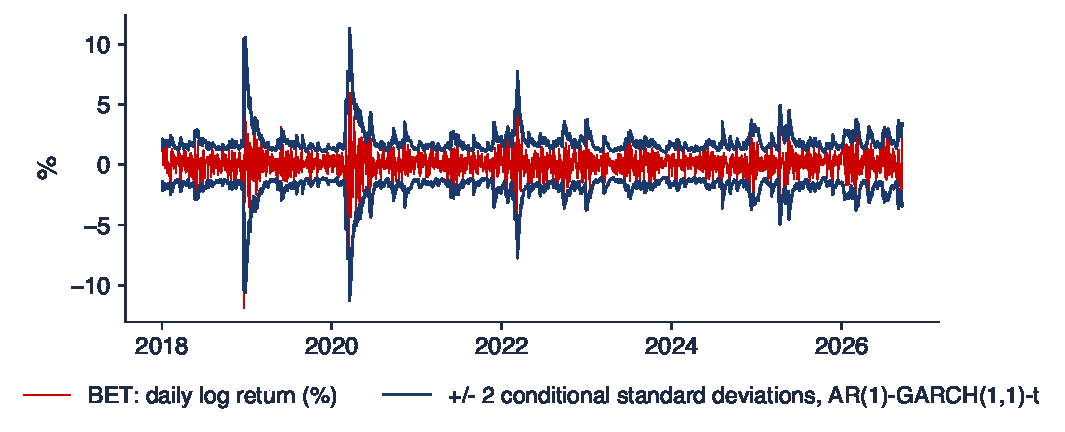
\includegraphics[width=0.96\textwidth,height=0.28\textheight,keepaspectratio]{ch5_sem_b1.pdf}
\end{center}
\vspace{-2mm}
\begin{center}
\scriptsize
\begin{tabular}{lrrrrrr}
\toprule
& $c$ & $\phi$ & $\omega$ & $\alpha$ & $\beta$ & $\nu$ \\
\midrule
estimare & $0{,}077$ & $0{,}091$ & $0{,}0441$ & $0{,}189$ & $0{,}801$ & $5{,}09$ \\
SE robustă & $0{,}010$ & $0{,}013$ & $0{,}0085$ & $0{,}023$ & $0{,}023$ & $0{,}32$ \\
\bottomrule
\end{tabular}
\end{center}
\begin{itemize}
    \item Reziduurile AR(1): ARCH-LM $= nR^2 = 1017$ ($R^2 = 0{,}153$), $Q(10)$ al pătratelor $= 2496$: efecte ARCH puternice
    \item $T = 6\,669$; $\alpha + \beta = 0{,}990$, timpul de înjumătățire $\ln 0{,}5/(-0{,}01028) = 67{,}4$ zile; volatilitatea de lungă durată 32{,}8\%, față de 22{,}1\% în eșantion; $\hat z_t$: $Q(10) = 28{,}6$ (p $<$\,0{,}001), $\hat z_t^2$: $7{,}2$ (p = 0{,}705)
    \item Vîrfuri: 114\% (2008), 89\% (2020); ultima zi: 26{,}2\%; 5{,}1\% dintre zile ies din banda $\pm 2\hat\sigma_t$
    \item Interpretare: sub nivelul de lungă durată (26{,}2\% față de 32{,}8\%); modelul se așteaptă ca volatilitatea să crească lent spre acest nivel, dar nivelul este imprecis ($1 - \alpha - \beta = 0{,}0102$)
\end{itemize}\quantlet{TSA\_ch5\_seminar}{\qlurl{TSA_ch5_seminar}}
\end{frame}

\begin{frame}{B2: EUR/RON și Bitcoin [Propus]}
\itemsize{\footnotesize}
\begin{itemize}
\item \textbf{Întrebarea}: se comportă cursul EUR/RON și Bitcoin la fel ca BET? Model: B1.
\item \textbf{Date}: EUR/RON (cursul de referință BNR) din iulie 2005, Bitcoin din septembrie 2014; randamente logaritmice zilnice în \%
\item \textbf{Cerințe}
\begin{enumerate}
    \item Repetați pașii 1--4 din B1 pentru ambele serii (EUR/RON: estimați pe $10\,r_t$).
    \item Raportați $\hat\alpha + \hat\beta$ și precizați dacă timpul de înjumătățire și volatilitatea de lungă durată există.
    \item Interpretare: ce înseamnă $\hat\alpha + \hat\beta = 1$ pentru o prognoză a volatilității peste un an?
\end{enumerate}
\item \textbf{Raportați}: un tabel și două fraze
\item Notebook: secțiunea B2
\end{itemize}
\end{frame}

\ifsolutions
\begin{frame}{B2: rezolvare [Propus]}
\itemsize{\footnotesize}
\begin{center}
\scriptsize
\begin{tabular}{lrrrrrrrrr}
\toprule
& $T$ & ARCH-LM & $\phi$ & $\alpha$ & $\beta$ & $\nu$ & $\alpha + \beta$ & vol. selecție & $Q(10)$, $\hat z_t^2$ \\
\midrule
EUR/RON & 5\,351 & 811 & $0{,}031$ & $0{,}122$ & $0{,}878$ & $4{,}21$ & $1{,}0000$ & 4{,}4 & $0{,}004$ \\
Bitcoin & 4\,383 & 106 & $-0{,}043$ & $0{,}106$ & $0{,}894$ & $3{,}15$ & $1{,}0000$ & 66{,}6 & $5{,}0$ \\
\bottomrule
\end{tabular}
\end{center}
\begin{itemize}
    \item Ambele: efecte ARCH puternice înainte de model; $\hat\alpha + \hat\beta = 1$ (IGARCH): fără timp de înjumătățire și fără volatilitate de lungă durată; cozi groase ($\hat\nu$ 4{,}21 și 3{,}15)
    \item EUR/RON: $\hat\phi = 0{,}031$ (OLS: 0{,}170): termenul AR aproape dispare cînd modelăm varianța; $Q(10)$ al lui $\hat z_t^2$ este foarte mic din cauza unei singure zile (6 mai 2025, Cursul 5)
    \item Interpretare: nu există revenire la medie: prognoza pentru orice orizont este egală cu varianța de mîine, ca la EWMA; o prognoză pe un an repetă pur și simplu nivelul de azi
\end{itemize}\quantlet{TSA\_ch5\_seminar}{\qlurl{TSA_ch5_seminar}}
\end{frame}
\fi

\begin{frame}{B3: efectul de levier la S\&P 500 [Rezolvat]}
\itemsize{\footnotesize}
\begin{itemize}
\item \textbf{Întrebarea}: cresc scăderile volatilitatea S\&P 500 mai mult decît creșterile de aceeași mărime?
\item \textbf{Date}: închiderile S\&P 500 din 2000, randamente logaritmice zilnice în \%
\item \textbf{Cerințe}
\begin{enumerate}
    \item Estimați GARCH(1,1)-t și GJR-GARCH(1,1)-t; raportați $\gamma$ cu statistica $t$ robustă.
    \item Calculați statistica LR pentru GJR față de GARCH, p-valoarea ei și cele două valori BIC.
    \item Aplicați testul de asimetrie (sign bias) pe reziduurile standardizate ale GARCH-t.
    \item Desenați ambele curbe de impact ale știrilor și calculați varianța GJR după șocuri de $-2\%$ și $+2\%$.
    \item Interpretare: cum schimbă efectul de levier VaR-ul din ziua de după o scădere?
\end{enumerate}
\item \textbf{Raportați}: patru statistici cu p-valori, două varianțe, graficul și două fraze
\item Notebook: secțiunea B3
\end{itemize}
\end{frame}

\begin{frame}{B3: rezolvare [Rezolvat]}
\itemsize{\scriptsize}
\begin{center}
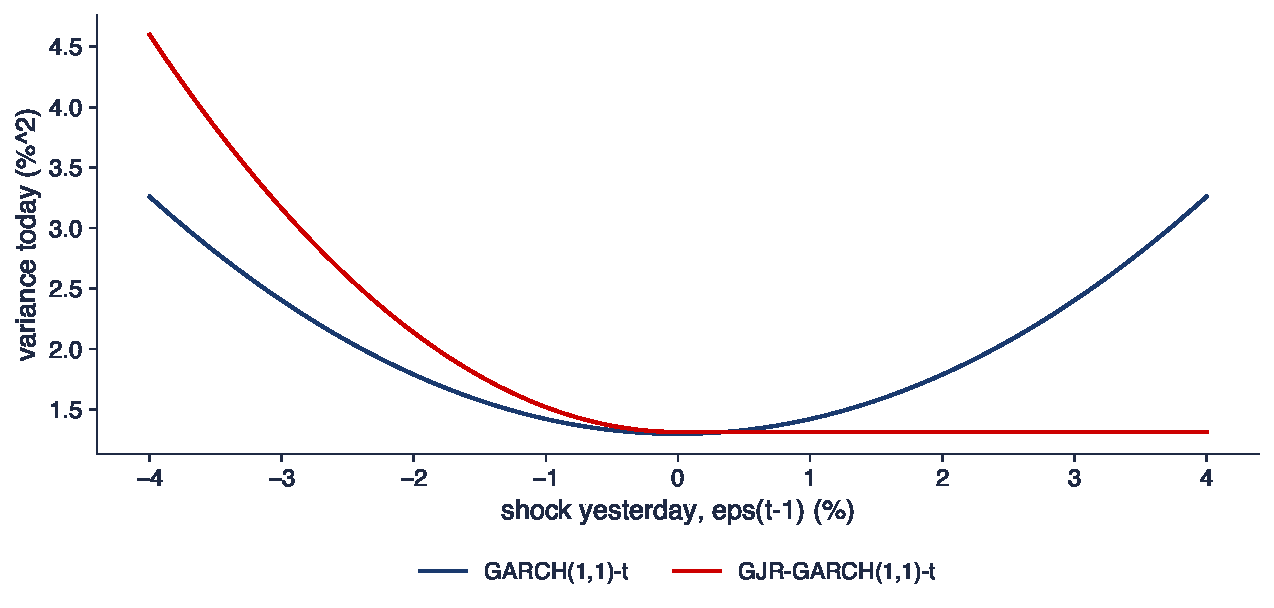
\includegraphics[width=0.96\textwidth,height=0.34\textheight,keepaspectratio]{ch5_sem_b3.pdf}
\end{center}
\vspace{-2mm}
\begin{itemize}
    \item GJR: $\hat\alpha = 0{,}000$, $\hat\gamma = 0{,}205$ ($t = 10{,}0$), $\hat\beta = 0{,}881$; LR $= 235{,}7$ (p $<$\,0{,}001); BIC $18169{,}0 \to 17942{,}2$
    \item Testul de asimetrie pe reziduurile GARCH-t: $\chi^2(3) = 40{,}7$ (p $<$\,0{,}001), $t$ al semnului $= 3{,}56$
    \item Varianța GJR după $-2\%$: $2{,}14$; după $+2\%$: $1{,}31$; raportul $1{,}62$
    \item Interpretare: doar scăderile cresc varianța ($\hat\alpha = 0$); după o scădere, VaR este de circa $\sqrt{1{,}62} = 1{,}27$ ori VaR-ul de după o creștere egală; un GARCH simetric subestimează riscul după zilele proaste
\end{itemize}\quantlet{TSA\_ch5\_seminar}{\qlurl{TSA_ch5_seminar}}
\end{frame}

\begin{frame}{B4: asimetria la BET, EUR/RON și Bitcoin [Propus]}
\itemsize{\footnotesize}
\begin{itemize}
\item \textbf{Întrebarea}: există un efect de levier la BET, la EUR/RON și la Bitcoin? Model: B3.
\item \textbf{Date}: BET din 2000, EUR/RON din 2005, Bitcoin din 2014; randamente logaritmice zilnice în \%
\item \textbf{Cerințe}
\begin{enumerate}
    \item Estimați GJR-GARCH(1,1)-t și EGARCH(1,1)-t; raportați ambele valori $\gamma$, cu statisticile $t$ robuste.
    \item Calculați testul LR pentru GJR față de GARCH și modificarea BIC.
    \item Interpretare: pentru EUR/RON un randament pozitiv înseamnă un leu mai slab; ce sînt „știrile proaste” pentru această serie?
\end{enumerate}
\item \textbf{Raportați}: un tabel și două fraze
\item Notebook: secțiunea B4
\end{itemize}
\end{frame}

\ifsolutions
\begin{frame}{B4: rezolvare [Propus]}
\itemsize{\footnotesize}
\begin{center}
\footnotesize
\begin{tabular}{lrrrrrrrr}
\toprule
& GJR $\alpha$ & GJR $\gamma$ & $t$ & LR & p & $\Delta$BIC & EGARCH $\gamma$ & $t$ \\
\midrule
BET & $0{,}172$ & $0{,}043$ & ${2{,}1}$ & $4{,}9$ & 0{,}026 & ${3{,}9}$ & ${-0{,}028}$ & ${-2{,}6}$ \\
EUR/RON & $0{,}103$ & $0{,}039$ & ${3{,}0}$ & $9{,}3$ & 0{,}002 & ${-0{,}7}$ & ${-0{,}040}$ & ${-2{,}5}$ \\
Bitcoin & $0{,}113$ & $-0{,}013$ & ${-0{,}7}$ & $0{,}7$ & 0{,}416 & ${7{,}7}$ & ${0{,}015}$ & ${1{,}2}$ \\
\bottomrule
\end{tabular}
\end{center}
\begin{itemize}
    \item BET: $\gamma > 0$ (în EGARCH $\gamma < 0$), semnificativ după testul LR la 5\%, dar BIC crește: un efect real, dar mic
    \item Bitcoin: nicio asimetrie ($t = -0{,}7$); EUR/RON: $\gamma > 0$ și semnificativ, cu BIC aproape neschimbat
    \item Interpretare: în GJR „știrile proaste” sînt $\varepsilon_{t-1} < 0$, zilele în care leul se întărește; pentru o valută semnul nu are sensul efectului de levier: o mișcare mare în orice direcție semnalează știri de politică monetară
\end{itemize}\quantlet{TSA\_ch5\_seminar}{\qlurl{TSA_ch5_seminar}}
\end{frame}
\fi

\begin{frame}{B5: GARCH față de EWMA pentru S\&P 500 [Rezolvat]}
\itemsize{\footnotesize}
\begin{itemize}
\item \textbf{Întrebarea}: prognozează GARCH(1,1)-t varianța de mîine a S\&P 500 mai bine decît EWMA și este VaR 1\% al lui depășit în 1\% dintre zile?
\item \textbf{Date}: S\&P 500 din 2000; prognoze pentru fiecare zi de la 2 ianuarie 2015
\item \textbf{Cerințe}
\begin{enumerate}
    \item Reestimați GARCH(1,1)-t la fiecare 250 de zile pe toate datele pînă în acea zi și calculați prognozele pe o zi $h_t$; calculați EWMA cu $\lambda = 0{,}94$.
    \item Calculați media QLIKE pentru ambele modele și statistica $t$ Diebold--Mariano.
    \item Numărați depășirile VaR 1\% GARCH-t și VaR 1\% EWMA-Normal și comparați-le cu numărul așteptat.
    \item Desenați diferența cumulată a pierderilor.
    \item Interpretare: ce model i-ați da unui manager de risc și ce ați mai îmbunătăți?
\end{enumerate}
\item \textbf{Raportați}: patru valori, două numărători, graficul și două fraze
\item Notebook: secțiunea B5
\end{itemize}
\end{frame}

\begin{frame}{B5: rezolvare [Rezolvat]}
\itemsize{\scriptsize}
\begin{center}
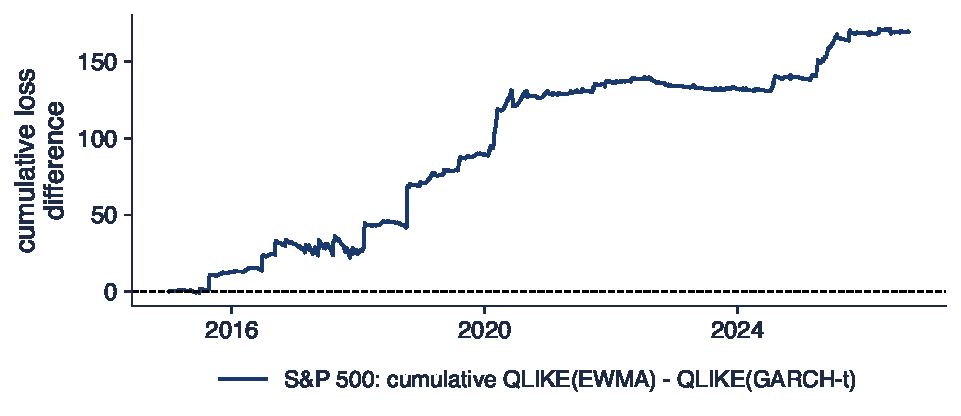
\includegraphics[width=0.96\textwidth,height=0.32\textheight,keepaspectratio]{ch5_sem_b5.pdf}
\end{center}
\vspace{-2mm}
\begin{itemize}
    \item 2\,944 de zile; media QLIKE: GARCH-t $0{,}761$, EWMA $0{,}819$; DM: diferența medie $-0{,}058$, $t = -3{,}69$ (p $<$\,0{,}001): GARCH-t este mai bun
    \item Depășiri VaR 1\%: GARCH-t 49 (1{,}66\%), EWMA-Normal 65 (2{,}21\%); așteptat circa 29
    \item Interpretare: GARCH-t, dar ambele modele VaR sînt depășite prea des; adăugăm efectul de levier (B3) și testăm formal numărul de depășiri (\refKupiec)
\end{itemize}\quantlet{TSA\_ch5\_seminar}{\qlurl{TSA_ch5_seminar}}
\end{frame}

\begin{frame}{B6: GARCH față de EWMA pentru BET și EUR/RON [Propus]}
\itemsize{\footnotesize}
\begin{itemize}
\item \textbf{Întrebarea}: se păstrează rezultatul din B5 pentru BET și pentru EUR/RON? Model: B5.
\item \textbf{Date}: BET din 2000, EUR/RON din 2005; prognoze pentru fiecare zi din ianuarie 2015
\item \textbf{Cerințe}
\begin{enumerate}
    \item Calculați prognozele GARCH(1,1)-t și EWMA în afara eșantionului, ca în B5.
    \item Calculați media QLIKE pentru ambele modele și testul DM.
    \item Găsiți ziua cu cea mai mare diferență a pierderilor și recalculați media QLIKE fără ea.
    \item Numărați depășirile VaR 1\% pentru ambele modele.
    \item Interpretare: de ce poate fi testul DM nesemnificativ cînd o medie QLIKE este jumătate din cealaltă?
\end{enumerate}
\item \textbf{Raportați}: un tabel și două fraze
\item Notebook: secțiunea B6
\end{itemize}
\end{frame}

\ifsolutions
\begin{frame}{B6: rezolvare [Propus]}
\itemsize{\footnotesize}
\begin{center}
\scriptsize
\begin{tabular}{lrrrrrrr}
\toprule
& QLIKE, GARCH-t & EWMA & DM $t$ (p) & ziua maximă & pondere & dep., GARCH-t & EWMA \\
\midrule
BET & $0{,}680$ & $0{,}788$ & ${-2{,}22}$ (0{,}027) & 19 decembrie 2018 & 39\% & 34 & 67 \\
EUR/RON & $2{,}456$ & $5{,}982$ & ${-1{,}02}$ (0{,}310) & 6 mai 2025 & 98\% & 35 & 63 \\
\bottomrule
\end{tabular}
\end{center}
\begin{itemize}
    \item Depășiri VaR 1\% așteptate: circa 29 pentru fiecare serie; BET: GARCH-t mai bun (DM $t = -2{,}22$), depășiri: 34, EWMA-Normal de circa două ori prea multe
    \item EUR/RON: media QLIKE 2{,}456 față de 5{,}982, dar DM $t = -1{,}02$: 98\% din diferență provine din 6 mai 2025; fără această zi: $-3{,}932$ față de $-3{,}877$
    \item Interpretare: statistica DM împarte diferența medie la eroarea ei standard; o singură pierdere enormă le mărește pe amîndouă, deci dovada se sprijină pe o zi și este slabă
\end{itemize}\quantlet{TSA\_ch5\_seminar}{\qlurl{TSA_ch5_seminar}}
\end{frame}
\fi


%=============================================================================
\section{Partea C: întrebări deschise și critica unui răspuns AI}
%=============================================================================

\begin{frame}{C1: este leul mai liniștit decît înainte? [Propus]}
\itemsize{\footnotesize}
\begin{itemize}
\item \textbf{Întrebarea}: s-a schimbat volatilitatea EUR/RON între perioadele 2005--2012, 2013--2019 și 2020--2026 și poate un singur model GARCH să descrie toate trei perioadele?
\item \textbf{Date}: randamentele logaritmice zilnice EUR/RON în \% (cursul de referință BNR); model: B1
\item \textbf{Cerințe}
\begin{enumerate}
    \item Pentru fiecare perioadă calculați volatilitatea de selecție anualizată și ponderea zilelor cu $|r_t| > 0{,}5\%$.
    \item Estimați GARCH(1,1)-t pe fiecare perioadă și raportați $\alpha + \beta$, $\alpha$ și $\nu$.
    \item Găsiți cea mai mare variație zilnică din fiecare perioadă și data ei.
    \item Interpretare: este schimbarea volatilității o proprietate a pieței sau a politicii de curs de schimb?
\end{enumerate}
\item \textbf{Raportați}: un tabel și un plan de proiect
\item Notebook: secțiunea C1
\end{itemize}
\end{frame}

\ifsolutions
\begin{frame}{C1: analiză de referință [Propus]}
\itemsize{\footnotesize}
\begin{center}
\scriptsize
\begin{tabular}{lrrrrrrr}
\toprule
Perioada & $T$ & vol.\ (\% pe an) & $|r| > 0{,}5\%$ (\%) & $\alpha + \beta$ & $\alpha$ & $\nu$ & max $|r|$ \\
\midrule
2005--2012 & 1\,908 & 6{,}7 & 15{,}4 & 1{,}000 & $0{,}195$ & $4{,}53$ & 2{,}93 \\
2013--2019 & 1\,761 & 3{,}0 & 2{,}4 & 1{,}000 & $0{,}109$ & $4{,}14$ & 1{,}71 \\
2020--2026 & 1\,683 & 1{,}7 & 0{,}7 & 1{,}000 & $0{,}187$ & $3{,}45$ & 1{,}42 \\
\bottomrule
\end{tabular}
\end{center}
\begin{itemize}
    \item Volatilitatea scade de la 6{,}7\% la 3{,}0\% și 1{,}7\% pe an; zilele cu variații mari, de la 15{,}4\% la 0{,}7\% dintre zile
    \item Fiecare perioadă este IGARCH ($\alpha + \beta = 1$), cu cozi foarte groase: perioade lungi de calm întrerupte de salturi rare (cele mai mari variații: 3 octombrie 2008, 7 iunie 2013, 19 mai 2025)
    \item Interpretare: nivelul este fixat de politica BNR, nu de piață; un GARCH cu parametri constanți nu se potrivește bine niciunei perioade; proiect: Markov switching (\tsachlink{https://danpele.github.io/Time-Series-Analysis/RO/Cursuri/capitol10_spatiul_starilor_kalman_markov_switching.pdf}{Capitolul 10}) sau un GARCH cu variabile de politică
\end{itemize}\quantlet{TSA\_ch5\_seminar}{\qlurl{TSA_ch5_seminar}}
\end{frame}
\fi

\begin{frame}{C2: verificați un răspuns AI [Propus]}
\itemsize{\scriptsize}
\begin{itemize}
    \item Un student a cerut unui asistent AI să interpreteze un GARCH(1,1)-t estimat pentru BET (date zilnice, din 2000): $\hat\omega = 0{,}0448$, $\hat\alpha = 0{,}192$, $\hat\beta = 0{,}799$, $\hat\nu = 5{,}01$. Răspunsul:
    \item \aiprompt{(a) Timpul de înjumătățire al unui șoc de volatilitate este ln 0,5 / ln beta = 3{,}1 zile.}
    \item \aiprompt{(b) Varianța de lungă durată este omega/(1 - alpha) = 0{,}055, o volatilitate anuală de 3{,}7\%.}
    \item \aiprompt{(c) Un AR(1) estimat prin OLS dă phi = 0{,}109 cu SE 0{,}012, t = 8{,}9: randamentele BET sînt puternic previzibile.}
    \item \aiprompt{(d) Ljung-Box Q(10) al pătratelor reziduurilor standardizate = 8{,}3, p = 0{,}60: modelul GARCH-t este corect.}
    \item \aiprompt{(e) Cu inovații Student-t, cuantila de 1\% a lui z este mai aproape de 0 decît valoarea Normală -2,326, deci VaR 1\% este mai mic.}
    \item \aiprompt{(f) alpha + beta = 0{,}991 < 1, deci modelul este staționar în covarianță, iar volatilitatea revine la nivelul de lungă durată.}
    \item Cerințe
    \begin{itemize}
        \item 1. Pentru fiecare afirmație, precizați dacă este corectă; dacă nu este, formulați afirmația corectă și, acolo unde se poate, dați valoarea corectă din notebook (secțiunea C2).
        \item 2. Raportați: o listă de șase verdicte, fiecare cu un rînd de justificare.
    \end{itemize}
\end{itemize}
\end{frame}

\ifsolutions
\begin{frame}{C2: rezolvare [Propus]}
\itemsize{\footnotesize}
\begin{itemize}
    \item (a) Greșit: timpul de înjumătățire folosește persistența, $\ln 0{,}5/\ln(\alpha + \beta) = \ln 0{,}5/\ln 0{,}991 = 74$ zile
    \item (b) Greșit: $\bar\sigma^2 = \omega/(1 - \alpha - \beta) = 4{,}82$, o volatilitate de lungă durată de 34{,}7\% (imprecisă, deoarece $1 - \alpha - \beta$ este mic)
    \item (c) Greșit: cu erori GARCH, SE din OLS este prea mică; SE robustă 0{,}029 ($t = 3{,}8$); AR(1)-GARCH-t: $\hat\phi = 0{,}091$ ($t = 6{,}8$); semnificativ, dar $\phi^2 \approx 0{,}012$ din varianță: o previzibilitate slabă
    \item (d) Greșit: nu a rămas niciun efect ARCH, dar asta nu dovedește că modelul este corect; $Q(10)$ al lui $\hat z_t$ este 114{,}6: a rămas autocorelație în medie (Cursul 5: AR(1)-GARCH)
    \item (e) Greșit: pentru $t$ standardizată cu $\nu = 5{,}01$ cuantila este $-2{,}606$, mai departe de 0 decît $-2{,}326$: VaR 1\% este mai mare
    \item (f) Corect
\end{itemize}\quantlet{TSA\_ch5\_seminar}{\qlurl{TSA_ch5_seminar}}
\end{frame}
\fi


%=============================================================================
\section{Încheiere}
%=============================================================================

\begin{frame}{Idei de reținut}
\itemsize{\small}
\begin{itemize}
    \item Testăm efectele ARCH pe reziduurile modelului pentru medie: ARCH-LM $= nR^2$ și Ljung--Box pe pătrate
    \item $\alpha + \beta$ decide termenul lung: timpul de înjumătățire, varianța de lungă durată, forma prognozelor; $\alpha + \beta = 1$: IGARCH
    \item Riscul pe mai multe zile este suma prognozelor zilnice ale varianței, nu $\sqrt{H}$ ori volatilitatea de azi
    \item Inovațiile cu cozi groase schimbă cuantila VaR; asimetria schimbă VaR-ul după zilele proaste
    \item Comparăm prognozele în afara eșantionului (QLIKE, DM) și căutăm zilele care determină singure rezultatul
\end{itemize}
\end{frame}

\begin{frame}{După seminar}
\itemsize{\small}
\begin{itemize}
    \item Cursul 5 dezvoltă fiecare temă de azi: faptele stilizate, ARCH și GARCH, estimarea, ARMA-GARCH, asimetria, diagnosticarea, prognozele, VaR 1\%
    \item Încercați cerințele [Propus] în notebook
    \item C1 poate deveni un proiect de echipă: regimurile de volatilitate ale leului și ale altor valute din regiune
    \item Lectură: \refHP, cap.~6; \refTsay, cap.~3
    \item \textbf{Seminarul are rol de exercițiu și nu se notează; rezolvările cerințelor [Propus] se discută la seminar}
\end{itemize}
\end{frame}


%=============================================================================
\section{Bibliografie}
%=============================================================================

\begin{frame}{Bibliografie}
\itemsize{\tiny}
\begin{itemize}
    \item Bollerslev, T. (1986). Generalized autoregressive conditional heteroskedasticity. \textit{Journal of Econometrics}, 31(3), 307--327. \href{https://doi.org/10.1016/0304-4076(86)90063-1}{doi:10.1016/0304-4076(86)90063-1}
    \item Bollerslev, T. (1987). A conditionally heteroskedastic time series model for speculative prices and rates of return. \textit{Review of Economics and Statistics}, 69(3), 542--547. \href{https://doi.org/10.2307/1925546}{doi:10.2307/1925546}
    \item Bollerslev, T., \& Wooldridge, J. M. (1992). Quasi-maximum likelihood estimation and inference in dynamic models with time-varying covariances. \textit{Econometric Reviews}, 11(2), 143--172. \href{https://doi.org/10.1080/07474939208800229}{doi:10.1080/07474939208800229}
    \item Christie, A. A. (1982). The stochastic behavior of common stock variances: Value, leverage and interest rate effects. \textit{Journal of Financial Economics}, 10(4), 407--432. \href{https://doi.org/10.1016/0304-405X(82)90018-6}{doi:10.1016/0304-405X(82)90018-6}
    \item Diebold, F. X., \& Mariano, R. S. (1995). Comparing predictive accuracy. \textit{Journal of Business \& Economic Statistics}, 13(3), 253--263. \href{https://doi.org/10.1080/07350015.1995.10524599}{doi:10.1080/07350015.1995.10524599}
    \item Engle, R. F. (1982). Autoregressive conditional heteroscedasticity with estimates of the variance of United Kingdom inflation. \textit{Econometrica}, 50(4), 987--1007. \href{https://doi.org/10.2307/1912773}{doi:10.2307/1912773}
    \item Engle, R. F., \& Ng, V. K. (1993). Measuring and testing the impact of news on volatility. \textit{Journal of Finance}, 48(5), 1749--1778. \href{https://doi.org/10.1111/j.1540-6261.1993.tb05127.x}{doi:10.1111/j.1540-6261.1993.tb05127.x}
    \item Glosten, L. R., Jagannathan, R., \& Runkle, D. E. (1993). On the relation between the expected value and the volatility of the nominal excess return on stocks. \textit{Journal of Finance}, 48(5), 1779--1801. \href{https://doi.org/10.1111/j.1540-6261.1993.tb05128.x}{doi:10.1111/j.1540-6261.1993.tb05128.x}
    \item Huang, C., \& Petukhina, A. (2022). \textit{Applied Time Series Analysis and Forecasting with Python}. Springer. \href{https://doi.org/10.1007/978-3-031-13584-2}{doi:10.1007/978-3-031-13584-2}
    \item J.P. Morgan/Reuters (1996). \textit{RiskMetrics -- Technical Document} (4th ed.). Morgan Guaranty Trust Company. \href{https://www.msci.com/documents/10199/5915b101-4206-4ba0-aee2-3449d5c7e95a}{msci.com}
    \item Kupiec, P. H. (1995). Techniques for verifying the accuracy of risk measurement models. \textit{Journal of Derivatives}, 3(2), 73--84. \href{https://doi.org/10.3905/jod.1995.407942}{doi:10.3905/jod.1995.407942}
    \item Ljung, G. M., \& Box, G. E. P. (1978). On a measure of lack of fit in time series models. \textit{Biometrika}, 65(2), 297--303. \href{https://doi.org/10.1093/biomet/65.2.297}{doi:10.1093/biomet/65.2.297}
    \item Nelson, D. B. (1991). Conditional heteroskedasticity in asset returns: A new approach. \textit{Econometrica}, 59(2), 347--370. \href{https://doi.org/10.2307/2938260}{doi:10.2307/2938260}
    \item Patton, A. J. (2011). Volatility forecast comparison using imperfect volatility proxies. \textit{Journal of Econometrics}, 160(1), 246--256. \href{https://doi.org/10.1016/j.jeconom.2010.03.034}{doi:10.1016/j.jeconom.2010.03.034}
    \item Tsay, R. S. (2010). \textit{Analysis of Financial Time Series} (3rd ed.). Wiley. \href{https://doi.org/10.1002/9780470644560}{doi:10.1002/9780470644560}
\end{itemize}
\end{frame}

\end{document}
